\documentclass[10pt,a4paper]{article}
\usepackage[margin=1.5cm,headheight=15pt]{geometry}
\usepackage[T1]{fontenc}
\usepackage{lmodern}
\usepackage{microtype}
\usepackage{amsmath,amssymb,mathtools}
\usepackage{xcolor}
\usepackage[skins,breakable]{tcolorbox}
\usepackage{enumitem,booktabs,tabularx,array,longtable}
\usepackage[explicit]{titlesec}
\usepackage{fancyhdr,lastpage}
\usepackage{tikz}
\usetikzlibrary{arrows.meta,positioning}
\usepackage{listings}
\usepackage{hyperref}
\definecolor{accent}{HTML}{2F3E9E}
\definecolor{ink}{HTML}{1B2030}
\definecolor{soft}{HTML}{5A6478}
\definecolor{good}{HTML}{1C7A52}
\definecolor{warn}{HTML}{B4560A}
\definecolor{idea}{HTML}{7A2E7A}
\hypersetup{colorlinks=true,linkcolor=accent,urlcolor=accent,
  pdftitle={CS5446 Week-by-Week Detailed Study Notes},
  pdfauthor={CS5446 Study Notes},bookmarksnumbered=true}
\color{ink}
\setlength{\parindent}{0pt}
\setlength{\parskip}{4pt}
\linespread{1.12}
\setlength{\emergencystretch}{2em}
\setlength{\abovedisplayskip}{5pt}
\setlength{\belowdisplayskip}{5pt}
\setlist[itemize]{leftmargin=1.4em,itemsep=3pt,topsep=4pt,parsep=0pt}
\setlist[enumerate]{leftmargin=1.6em,itemsep=3pt,topsep=4pt,parsep=0pt}
\renewcommand{\arraystretch}{1.18}
\newcolumntype{P}[1]{>{\raggedright\arraybackslash}p{#1}}
\newcolumntype{Y}{>{\raggedright\arraybackslash}X}
\pagestyle{fancy}\fancyhf{}
\lhead{\small\color{soft}CS5446 \; Reinforcement Learning}
\rhead{\small\color{soft}Weeks 1--7 | Detailed Study Notes}
\cfoot{\small\color{soft}\thepage\,/\,\pageref{LastPage}}
\renewcommand{\headrulewidth}{0.3pt}
\titleformat{\section}{\Large\bfseries\color{accent}}{}{0pt}{\thesection\quad #1}
\titleformat{name=\section,numberless}{\Large\bfseries\color{accent}}{}{0pt}{#1}
\titleformat{\subsection}{\large\bfseries\color{accent}}{}{0pt}{#1}
\titlespacing*{\section}{0pt}{12pt}{6pt}
\titlespacing*{\subsection}{0pt}{8pt}{4pt}
\tcbset{studybox/.style={enhanced,breakable,arc=2pt,boxrule=0.6pt,
  left=7pt,right=7pt,top=5pt,bottom=5pt,boxsep=1pt,
  before skip=6pt,after skip=6pt,lines before break=4,fonttitle=\bfseries\small,coltitle=white}}
\newtcolorbox{card}[1]{studybox,colback=white,colframe=accent!70,colbacktitle=accent,title={#1}}
\newtcolorbox{idea}[1][Intuition]{studybox,colback=idea!5,colframe=idea!50,colbacktitle=idea!80,title={#1}}
\newtcolorbox{note}[1][Common Pitfalls]{studybox,colback=warn!5,colframe=warn!50,colbacktitle=warn!85,title={#1}}
\newtcolorbox{prf}[1][Derivation / Proof]{studybox,colback=good!4,colframe=good!50,colbacktitle=good!85,title={#1}}
\newtcolorbox{question}[1]{studybox,colback=idea!3,colframe=idea!65,colbacktitle=idea!85,title={#1}}
\newtcolorbox{plain}{studybox,colback=accent!4,colframe=accent!35}
\newcommand{\key}[1]{\textbf{\color{accent}#1}}
\newcommand{\ans}{\par\smallskip\textbf{\color{good}Solution\quad}}
\newcommand{\pit}{\par\smallskip\textbf{\color{warn}Note\quad}}
\newcommand{\E}{\mathbb E}
\newcommand{\Var}{\operatorname{Var}}
\newcommand{\argmax}{\operatorname*{arg\,max}}
\newcommand{\argmin}{\operatorname*{arg\,min}}
\newcommand{\clip}{\operatorname{clip}}
\newcommand{\Pre}{\operatorname{Pre}}
\newcommand{\Add}{\operatorname{Add}}
\newcommand{\Del}{\operatorname{Del}}
\newcommand{\Reach}{\operatorname{REACH}}
\newcommand{\ind}{\mathbf 1}
\newcommand{\topic}[1]{\clearpage\section{#1}}
\lstset{basicstyle=\ttfamily\footnotesize,columns=fullflexible,
  keepspaces=true,breaklines=true,showstringspaces=false,
  frame=none,aboveskip=4pt,belowskip=4pt}
\setcounter{tocdepth}{2}
\begin{document}

{\LARGE\bfseries\color{accent}CS5446\quad Week-by-Week Study Notes}\par
{\large Reinforcement Learning and Sequential Decision Making}\par

\begin{plain}
\textbf{How to read this revision.} Each week starts with the decision question, then builds the mechanism, and only then applies the equations. The worked questions are practice, not new definitions. When a symbol changes role between sections (especially $G$, $r$, and $\pi$), the local definition takes priority. Core headings follow the supplied course overview and lecture slides; optional mathematical extensions and decision-tree rollback are kept brief and marked as such.

\textbf{Lecture map:} Week 1 --- Course Overview, Introduction, Classical (Symbolic) Planning; Week 2 --- Real World Planning and Acting; Week 3 --- Rational Decision Making Utility Theory; Week 4 --- Markov Decision Process and Sequential Decision Making under Uncertainty; Week 5 --- Model-Free Techniques; Week 6 --- Reward Shaping for Reinforcement Learning and Its Applications (guest lecture); Week 7 --- the Course Overview's MCTS/UCT and imitation-learning topics. The supplied additional-notes PDFs support selected examples but do not set the main outline.
\end{plain}

\tableofcontents




\section*{Quick Reference}
\addcontentsline{toc}{section}{Quick Reference}
\begin{card}{A four-step routine for numerical questions}
\begin{enumerate}
\item \textbf{State the question before calculating.} Is the target a fixed-policy value, an optimal value, a sampled return, a TD update, or a policy-gradient objective? Identify the current state, chosen action, successor, and terminal status.
\item \textbf{Write the relevant equation and timing.} Distinguish an expectation over successor states $P(s'\mid s,a)$, a policy average over actions $\pi(a\mid s)$, and a maximum over actions. Check whether reward is paid on entry and whether the old or newly updated estimates are used.
\item \textbf{Substitute in separate stages.} Compute a model probability or continuation value first; then target or return; then TD error; then new estimate or maximizing action. Keep a fixed policy fixed during evaluation.
\item \textbf{Sanity-check the result.} Transition probabilities sum to one; a terminal continuation is zero; a return discounts later rewards once per step; a learning update moves toward its target; a greedy action compares values for the \emph{same state}.
\end{enumerate}
\end{card}
\begin{card}{First identify the decision problem}
\small
\par\smallskip
\begin{tabularx}{\linewidth}{@{}P{2.4cm}Y Y@{}}
\toprule Problem & Known information / objective & Methods \\\midrule
Classical planning & Known deterministic model; find a goal-reaching action sequence & STRIPS, progression, regression, SATPlan \\
Hierarchical planning & Primitive actions and method library; find an executable refinement & HTN, HLA, reachable sets \\
One-shot decision & Probabilities and preferences; maximize expected utility & MEU, Bayes, decision tree \\
MDP planning & Known $P,R$; maximize long-term return & VI, PI, Bellman equations \\
RL prediction & Fixed $\pi$, unknown model; estimate $V^\pi$ & ADP, MC, TD \\
RL control & Improve $\pi$; explore and learn good decisions & Active ADP, MC control, SARSA, Q-learning \\
Large-state RL & Tables are impractical; generalize with shared parameters & Function approximation, DQN, PG, PPO \\
Guided decisions & Simulator or expert data available & Rollout, MCTS; BC, DAgger, GAIL \\\bottomrule
\end{tabularx}\par\smallskip
\end{card}
\begin{card}{Notation and reward timing}
$s,a,s'$: current state, action, successor; $P(s'\mid s,a)$: transition probability; $r=R(s,a,s')$: reward for this transition. $\alpha$ is the \textbf{learning rate}; $\gamma$ is the \textbf{discount factor}.
\[
G_t=\sum_{k=0}^{H-1}\gamma^kR_{t+k+1},\qquad
V^\pi(s)=\E_\pi[G_t\mid S_t=s],\quad
Q^\pi(s,a)=\E_\pi[G_t\mid S_t=s,A_t=a].
\]
$G_t$ is a realized trajectory return; $V,Q$ are expectations. $V^*,Q^*$ are optimal; $\hat V,\hat Q$ are estimates. $Q^\pi$ forces action $a$ first, then follows $\pi$.

\textbf{Course default: reward on entry}, $R(s,a,s')=f(s')$. A problem may instead specify $R(s,a)$ (as in Nova). $R(s,a,s')=f(s)$ is also valid; keep one convention throughout each problem. Tutorial 4 writes the reward after $a_t$ as $r_t$, equivalent to $R_{t+1}$ here.

\textbf{True termination:} pay the terminal payoff upon entry, then set $V(T)=0$. An artificial time-limit truncation need not be true termination; a continuing task usually still requires bootstrapping.
\end{card}
\begin{card}{Value updates: identify the target, then compute the error}
\[
\boxed{\text{new estimate}=\text{old estimate}+\alpha(\text{target}-\text{old estimate})}
\]
\small
\par\smallskip
\begin{tabularx}{\linewidth}{@{}P{3cm}Y@{}}
\toprule Method & Target / actor weight \\\midrule
MC & $G_t$: complete episode return \\
TD(0) & $r+\gamma V(s')$ \\
SARSA & $r+\gamma Q(s',a')$; $a'$ is the action actually selected by the behavior policy \\
Q-learning & $r+\gamma\max_bQ(s',b)$ \\
DQN & $r+\gamma\max_bQ_{\theta^-}(s',b)$; fixed target network \\
Policy evaluation & $\sum_{s'}P(s'\mid s,\pi(s))[R+\gamma V(s')]$ \\
VI & $\max_a\sum_{s'}P(s'\mid s,a)[R+\gamma V(s')]$ \\
REINFORCE actor & $G_t$ or $G_t-b(s_t)$, multiplying the score gradient \\
TD Actor-Critic actor & $\delta_t=r+\gamma V_w(s')-V_w(s)$ as an advantage estimate \\\bottomrule
\end{tabularx}\par\smallskip
The bootstrap term is zero for a terminal transition.
\end{card}
\begin{note}[A consistent format for numerical updates]
Write \textbf{old value} $\to$ \textbf{target} (using the specified pre-update values) $\to$ \textbf{error} $\to$ \textbf{multiply by $\alpha$} $\to$ \textbf{new value}. With a known model, average over all outcomes; a single-sample update changes only its specified entry or parameters.
\end{note}

\topic{Week 1: Responsible Agents and Classical Planning}



\subsection{Start with the agent, task, and performance measure}
\begin{card}{From a task environment to a decision model}
An agent senses an environment, maintains a representation, selects an action, and observes its consequences. A rational choice maximizes the stated performance criterion given available information; a good decision can still have a bad stochastic outcome.
\begin{enumerate}
\item Specify the objective: goal satisfaction, minimum cost, expected utility, or long-term reward. They are different optimization problems.
\item Choose a sufficient state description: retain facts needed to determine legal actions and consequences; omit irrelevant detail.
\item Specify actions and effects. A symbolic model explicitly encodes them; RL can learn from interaction when they are unknown.
\item Distinguish a \textbf{plan} (an action sequence) from a \textbf{policy} (a rule selecting actions from current states). A deterministic open-loop plan suffices only under the appropriate assumptions; uncertainty often requires feedback.
\end{enumerate}
Fully observable means the current state can be determined. Deterministic means the next state is fixed by the current state and action. Static means the relevant world does not evolve independently while planning. These assumptions are independent.
\end{card}

\begin{idea}[Why responsible planning belongs in the model]
A delivery agent can optimize travel time while violating a safety constraint. First identify stakeholders and harms; then decide which are hard constraints (never enter a forbidden area) and which are trade-offs (time versus energy). Transparency concerns whether the choice can be explained; accountability concerns who is responsible for deployment and failure. Maximizing a numerical reward does not by itself establish that the objective is appropriate.
\end{idea}

\subsection{Represent states, actions, and goals in STRIPS / PDDL}
\begin{card}{Planning problem, state, goal, action}
$\mathcal P=\langle S,s_0,A,T,G\rangle$. A plan is an action sequence that reaches $G$ from $s_0$; a valid plan need not have minimum cost.

\textbf{Classical assumptions:} known model, fully observable, deterministic, static, discrete, and usually single-agent.
\begin{itemize}
\item A state is a set of true ground atoms. \textbf{Closed world:} absent atoms are false; distinct object names denote distinct objects.
\item A schema contains variables; grounding substitutes objects for them. Static type facts are normally preserved by all actions.
\item A goal is a \textbf{partial description}: $G^+\subseteq s$ and $G^-\cap s=\varnothing$; it need not specify the entire state.
\item $a$ is applicable iff $\Pre^+(a)\subseteq s$ and $\Pre^-(a)\cap s=\varnothing$; then apply
\[
\boxed{T(s,a)=(s\setminus\Del(a))\cup\Add(a).}
\]
\item \textbf{Frame / inertia:} facts absent from the effects remain unchanged. Check invariants such as one location per object and a clear table against the actual model.
\end{itemize}
The domain specifies requirements, types, predicates, and action schemas. The problem specifies the domain, objects, initial state, and goal. Declare requirements for features such as equality and typing.
\end{card}

\begin{plain}
\textbf{T1 slides: logic quick reference.} $A$ is a constant; $x$ a variable; $On/2$ a binary predicate symbol; $On(x,y)$ an atom with variables; $On(A,B)$ a ground atom; $\neg Clear(B)$ a negative literal.
$\land$: both; $\lor$: at least one; $\neg$: negation; $\forall x$: every $x$; $\exists x$: at least one $x$. $A\ne B$ compares objects, not predicates.
\end{plain}

\begin{card}{Schema counts are not applicability counts}
For $n_p$ planes and $n_a$ airports, Fly$(p,from,to)$ has $n_pn_a^2$ type-correct instances if equal endpoints are allowed. If $from\ne to$ is explicitly required, the count is $n_pn_a(n_a-1)$. A type-correct instance may still be inapplicable in the current state. Grounding restricts objects; applicability checks state conditions.

For $n_c$ cargos, Load$(c,p,a)$ has $n_cn_pn_a$ typed instances; only cargo and plane pairs actually colocated at $a$ can load. CWA does not mean that an omitted effect becomes false: absent facts in a state are false, while facts absent from an action's effects persist.
\end{card}

\begin{question}{T5 Q1(a,b): Air Cargo grounding and applying effects}\label{q:t5q1}
\textbf{Schemas:} Load$(c,p,a)$ requires $At(c,a),At(p,a),Cargo(c),Plane(p),Airport(a)$; it deletes $At(c,a)$ and adds $In(c,p)$. Fly$(p,fr,to)$ requires $At(p,fr),Plane(p),Airport(fr),Airport(to)$; it deletes $At(p,fr)$ and adds $At(p,to)$. \textbf{There is no $fr\ne to$ condition.}

\textbf{(a)} Given $At(P_1,JFK),At(P_2,SFO)$ and all plane / airport facts, list every applicable Fly action.
\ans Four: $Fly(P_1,JFK,JFK)$, $Fly(P_1,JFK,SFO)$, $Fly(P_2,SFO,JFK)$, $Fly(P_2,SFO,SFO)$. Self-flights are unhelpful but satisfy the schema; do not omit them.

\textbf{(b)} Use the figure's initial state: $At(C_1,SFO),At(C_2,JFK),At(P_1,SFO),At(P_2,JFK)$, plus the type facts for both cargos, planes, and airports. Execute $Load(C_2,P_2,JFK)$.
\ans All preconditions hold; $s'=(s_0\setminus\{At(C_2,JFK)\})\cup\{In(C_2,P_2)\}$. All other location and type facts persist.
\pit The planes' locations in (a) are reversed relative to the figure in (b). Use each subquestion's own state.
\end{question}

\subsection{Search forward through states or backward through goals}
\begin{card}{Forward states and backward goal descriptions}
\small
\par\smallskip
\begin{tabularx}{\linewidth}{@{}P{2.3cm}Y Y@{}}
\toprule & Progression & Regression \\\midrule
Start / node & $s_0$; complete state & Goal; partial conditions \\
Action test & Applicable & Relevant: achieves a goal literal without destroying another requirement \\
Update & $(s\setminus\Del)\cup\Add$ & Positive-goal STRIPS: $(G\setminus\Add(a))\cup\Pre(a)$ \\
Stop & Current state satisfies goal & $s_0$ satisfies regressed conditions \\\bottomrule
\end{tabularx}\par\smallskip
\textbf{Positive-goal action test.} $\Add(a)\cap G\ne\varnothing$ asks whether $a$ achieves at least one currently required fact. $\Del(a)\cap G=\varnothing$ asks whether it destroys any currently required fact. The empty intersection means \emph{no conflict}; it does not mean the delete list or the goal is empty. After passing both tests, regress by replacing achieved facts with the action's preconditions. Negative goals require the more general rule below.

With $n$ Boolean fluents there are up to $2^n$ complete states, because each fluent is true or false. A partial goal has three possibilities per fluent---required true, required false, or unspecified---so there are up to $3^n$ descriptions. These are possible representations, not a prediction of how many search nodes will actually be expanded.
\end{card}

\begin{idea}[Lecture example: Move and HasKey]
$s_0=\{AtA,HasKey\}$, $G=\{AtB,HasKey\}$; Move has Pre$=\{AtA\}$, Add$=\{AtB\}$, Del$=\{AtA\}$.
Forward gives $\{AtB,HasKey\}$; regression gives $\{AtA,HasKey\}$. HasKey remains a required goal condition even though it is not a Move precondition.
\end{idea}

\begin{card}{Regression with positive and negative literals}
Represent a goal by $(G^+,G^-)$: facts in $G^+$ must be true and facts in $G^-$ must be false. A useful action must establish at least one still-required positive or negative literal. It may not delete a required positive fact or add a forbidden fact:
\[
\bigl(\Add(a)\cap G^+\bigr)\cup\bigl(\Del(a)\cap G^-\bigr)\ne\varnothing,
\quad \Del(a)\cap G^+=\varnothing,\quad \Add(a)\cap G^-=\varnothing.
\]
Then ask what would have had to be true \emph{before} that action:
\[
G'^+=(G^+\setminus\Add(a))\cup\Pre^+(a),\quad
G'^-=(G^-\setminus\Del(a))\cup\Pre^-(a).
\]
Reject if $G'^+\cap G'^-\ne\varnothing$: the same fact cannot simultaneously be required true and false. Stop when $G'^+\subseteq s_0$ and $G'^-\cap s_0=\varnothing$. The first condition checks that all required positives are initially present; the second checks that none of the forbidden facts is initially present. Extra initial facts are allowed, provided they are not forbidden.

\textbf{Example:} $G^+=\{Delivered\}$, $G^-=\{Loaded\}$; Unload requires Loaded and AtDest, adds Delivered, deletes Loaded. Regression yields $G'^+=\{Loaded,AtDest\}$, $G'^-=\varnothing$. Loaded must be true before Unload even though false afterward.
\end{card}

\begin{card}{Search and correctness: key distinctions}
BFS finds the fewest steps with finite branching and equal step costs; UCS handles differing nonnegative costs. A* uses $g+h$; admissibility means $0\le h\le h^*$. Graph search without reopening generally needs consistency: $h(s)\le c(s,a)+h(s')$.

\textbf{Sound:} returned plans are valid. \textbf{Complete:} finds a plan whenever one exists. \textbf{Optimal:} minimizes the specified cost. General finite propositional STRIPS plan existence is PSPACE-complete; existence with a \textbf{polynomial length bound} is typically NP-complete. Distinguish bounded from unbounded planning.
\end{card}

\begin{question}{T1 P1(a--c): Middle-pop Blocks World}\label{q:t1p1}
\textbf{Problem:} initially a tower $A/B/C$ ($A$ on top, $C$ on Table). Move the middle block $B$ onto Table and end with $A$ on $C$. The only objects are $A,B,C,Table$; Table cannot move and always has space. Write PDDL, draw a forward search tree, and give a valid plan.
\ans Use separate actions for moving onto a block and onto Table. $x\ne fr$, $x\ne to$, and $fr\ne to$ exclude self-stacking and redundant moves. Table is an object, not a block.
\begin{lstlisting}
(define (domain middle-pop)
  (:requirements :strips :typing :equality)
  (:types block)
  (:constants Table - object)
  (:predicates (on ?x - block ?y - object) (clear ?x - object))
  (:action move-to-block
    :parameters (?x - block ?fr - object ?to - block)
    :precondition (and (on ?x ?fr) (clear ?x) (clear ?to)
      (not (= ?x ?fr)) (not (= ?x ?to)) (not (= ?fr ?to)))
    :effect (and (not (on ?x ?fr)) (on ?x ?to)
      (clear ?fr) (not (clear ?to))))
  (:action move-to-table
    :parameters (?x - block ?fr - block)
    :precondition (and (on ?x ?fr) (clear ?x) (not (= ?x ?fr)))
    :effect (and (not (on ?x ?fr)) (on ?x Table) (clear ?fr))))
(define (problem middle-pop-instance)
  (:domain middle-pop)
  (:objects A B C - block)
  (:init (on A B) (on B C) (on C Table) (clear A) (clear Table))
  (:goal (and (on B Table) (on A C))))
\end{lstlisting}
Table cannot be a \texttt{move-to-block} destination, so $Clear(Table)$ is never deleted. Inertia preserves $Clear(x)$ for the moved block.
\ans The only useful applicable action at $s_0$ is $MoveToTable(A,B)$. Then $A$ is on Table and $B/C$ remains stacked. The next layer has three successors:
\begin{center}
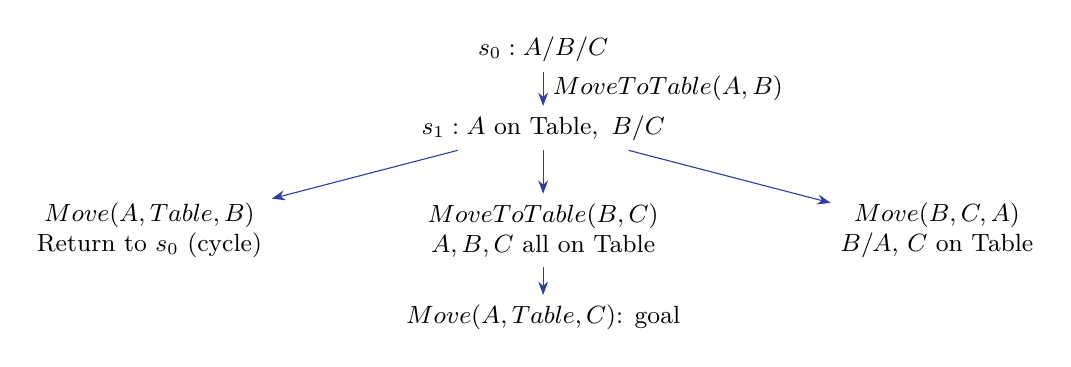
\begin{tikzpicture}[every node/.style={font=\small,align=center},edge/.style={-{Stealth},draw=accent}]
\node (r) at (0,0) {$s_0: A/B/C$};
\node (m) at (0,-1.0) {$s_1: A\text{ on Table},\ B/C$};
\node (l) at (-5,-2.3) {$Move(A,Table,B)$\\Return to $s_0$ (cycle)};
\node (c) at (0,-2.3) {$MoveToTable(B,C)$\\$A,B,C$ all on Table};
\node (rr) at (5,-2.3) {$Move(B,C,A)$\\$B/A$, $C$ on Table};
\node (g) at (0,-3.4) {$Move(A,Table,C)$: goal};
\draw[edge] (r)--node[right] {$MoveToTable(A,B)$}(m);
\draw[edge] (m)--(l);\draw[edge] (m)--(c);\draw[edge] (m)--(rr);\draw[edge] (c)--(g);
\end{tikzpicture}
\end{center}
Full forward search repeatedly generates all applicable actions and prunes duplicate states. The diagram shows the first two layers and the solution branch.
\[
\boxed{[MoveToTable(A,B),\ MoveToTable(B,C),\ Move(A,Table,C)]}
\]
Three actions are minimal in this model: clear $B$ by moving $A$, move $B$, then put $A$ onto $C$.
\end{question}

\begin{idea}[Why a yes/no planning problem can use polynomial space]
The question ``Does \emph{some} plan exist?'' asks for one bit of output, but finding that bit may require searching a very long sequence. A planner can traverse the implicit graph of up to exponentially many states while keeping only a current state, counters, and a search stack of polynomial size. Thus unbounded propositional plan existence can be PSPACE-complete even though the answer is only yes or no. If the plan length is bounded by a polynomial supplied as part of the decision problem, a candidate sequence can be guessed and checked in polynomial time; this is the usual NP-complete bounded version. Output size and search space are different issues.
\end{idea}

\subsection{Encode a bounded plan as SAT}
\begin{card}{Five constraint types and horizon search}
Create fluent variables for $t=0,\ldots,H$ and action variables for $t=0,\ldots,H-1$. Encode \textbf{initial truths / falsities, goal, action preconditions / effects, frame / successor-state axioms, and mutex / action exclusivity}. Increase $H$; when satisfiable, extract the actions and replay them to validate the plan.
\[
F_{t+1}\leftrightarrow
\bigvee_{a:F\in\Add(a)}a_t\ \lor\
\left(F_t\land\neg\bigvee_{a:F\in\Del(a)}a_t\right).
\]
Read $\bigvee$ as ``at least one of these actions.'' The first term says an action made $F$ true; the second says it was already true and no action deleted it. The $\land$ joins conditions that must both hold. The equation also rules out $F$ becoming true spontaneously.

The first satisfiable horizon in a serial encoding gives the \textbf{fewest steps}, not necessarily minimum weighted cost. Parallel encoding may minimize makespan and must handle interference correctly.
\end{card}

\begin{idea}[Lecture example: Cake, a two-step plan]
Initial state: $\neg Have_0\land\neg Eaten_0$; goal: $\neg Have_2\land Eaten_2$.
\[
\begin{aligned}
Eat_t&\Rightarrow Have_t\land\neg Have_{t+1}\land Eaten_{t+1},\\
Bake_t&\Rightarrow\neg Have_t\land Have_{t+1},\\
Have_{t+1}&\leftrightarrow Bake_t\lor(Have_t\land\neg Eat_t),\\
Eaten_{t+1}&\leftrightarrow Eat_t\lor Eaten_t,\quad
\neg Eat_t\lor\neg Bake_t.
\end{aligned}
\]
$H=1$ is infeasible; $H=2$ yields Bake, Eat. Implications alone are insufficient: Eaten could otherwise appear without a cause.
\end{idea}

\begin{card}{SAT encoding: implication to CNF and model extraction}
An action variable $a_t$ represents execution during $t\to t+1$. The precondition rule is $a_t\Rightarrow p_t$, equivalently $\neg a_t\lor p_t$. This forbids exactly one assignment: action true while precondition false. It does \emph{not} require the action whenever $p_t$ happens to be true. An add effect $q$ gives $\neg a_t\lor q_{t+1}$; a delete effect $r$ gives $\neg a_t\lor\neg r_{t+1}$.

For the Cake example, $Eaten_{t+1}\leftrightarrow(Eat_t\lor Eaten_t)$ becomes
\[
(\neg Eaten_{t+1}\lor Eat_t\lor Eaten_t)
\land(\neg Eat_t\lor Eaten_{t+1})
\land(\neg Eaten_t\lor Eaten_{t+1}).
\]
The first clause forbids spontaneous truth; the other two enforce creation and persistence. Initial-state clauses specify both true and false fluents. ``At most one action'' adds pairwise mutex clauses $\neg a_t\lor\neg b_t$; ``exactly one'' also requires $\bigvee_a a_t$. Permit idle steps or no-ops when appropriate to the horizon convention.

UNSAT at horizon $H$ rules out that bounded encoding only. It does not rule out longer plans. SAT gives an assignment; extract true action variables, order by time, and replay preconditions and effects.
\end{card}

\begin{note}[Brief reference: LFM-assisted / responsible planning]
An LFM can generate or repair models, split subgoals, provide heuristics, and propose reusable strategies; symbolic validation is still needed. For responsible planning, use \textbf{stakeholder $\to$ risk $\to$ mitigation $\to$ trade-off}. Recognize safety, privacy, fairness, transparency, accountability, and human oversight. Case timelines and tool lists are omitted.
\end{note}

\begin{question}{Week 1 self-check}
Why are precondition/effect implications alone insufficient for SATPlan? Why can regression preserve a fact absent from the selected action's preconditions?
\ans Implications constrain what happens if an action executes, but do not prevent unconstrained facts appearing without an action; frame or successor-state axioms supply this restriction. Regression preserves unmet goals because the selected action neither establishes nor destroys them: earlier actions must make them true.
\end{question}

\topic{Week 2: Planning and Acting in Complex Environments}



\subsection{Guide search with relaxed and abstract models}
\begin{card}{Heuristic guidance, pruning, and abstraction have different roles}
A heuristic orders exploration; pruning removes branches; abstraction replaces detailed states with a smaller representation. A poor but admissible heuristic can be slow. A useful inadmissible heuristic can find good solutions quickly without guaranteeing minimum cost. Unsafe pruning may destroy completeness even when the heuristic is admissible.

A* orders by $g+h$ (cost so far plus estimated remaining cost); greedy best-first search orders by $h$ only. SAT/CSP planners usually use internal branching and propagation heuristics rather than an explicit goal-distance $h(s)$.
\end{card}

\begin{card}{Admissibility and heuristic comparison}
Relax constraints while retaining action costs and all original solutions. Thus $h^*_{relaxed}\le h^*_{original}$. The \textbf{exact relaxed optimum} is a lower bound; the cost of an arbitrary relaxed plan need not be.
\small
\par\smallskip
\begin{tabularx}{\linewidth}{@{}P{2.3cm}Y P{3.7cm}@{}}
\toprule Heuristic & Construction & Admissible? \\\midrule
Misplaced tiles & Remove Blank and Adjacent preconditions; each misplaced tile needs a move & Yes for standard unit-cost puzzles \\
Manhattan & Remove Blank, retain Adjacent; sum tile grid distances & Yes for standard puzzles; exclude blank \\
$h_{max}$ & Maximum of goal / precondition costs & Yes when components are lower bounds \\
$h_{add}$ & Sum costs, ignoring shared actions & Generally no: may double-count \\
$h^+$ & Optimal delete-relaxed plan cost & Yes for positive STRIPS; hard to compute \\
$h_{FF}$ & Greedily extracted relaxed plan & Generally no: extraction need not be optimal \\\bottomrule
\end{tabularx}\par\smallskip
\normalsize
Initialize relaxed fact costs: $c(p)=0$ if $p\in s$, otherwise $\infty$; update to a fixed point:
\[
c_{max}(p)=\min_{a:p\in\Add(a)}\left[c(a)+\max_{q\in\Pre(a)}c_{max}(q)\right].
\]
Replace the inner max with a sum for $c_{add}$; aggregate goal costs using max / sum. Empty preconditions contribute zero.
\end{card}

\begin{note}[Common max / sum pitfall]
One unit-cost action adds both $p,q$; goal $p\land q$. Then $h^*=h^+=h_{max}=1$, but $h_{add}=2$. The max of admissible estimates is admissible; a sum needs independence or valid cost partitioning. Manhattan is admissible for the 8-puzzle because each move shifts exactly one numbered tile one square; this is not a general rule.
\end{note}

\begin{card}{Abstraction and admissibility: what must be preserved}
Let $f:S\to\bar S$. For a lower-bound heuristic, concrete goal states must map to abstract goals, and concrete transitions must map to abstract transitions or paths with no greater cost. Every concrete solution then induces an abstract solution, so the abstract optimal cost cannot be larger. An arbitrary grouped problem is not automatically admissible.

A pattern database stores exact distances in a selected abstraction. Taking the maximum of several admissible databases is safe. Adding them needs a proof that action costs are not counted repeatedly, usually via cost partitioning.

\textbf{Air Cargo counting (lecture):} ignoring additional constraints, 50 planes have $10^{50}$ location assignments; each of 200 cargos has 50 plane or 10 airport locations, giving $10^{50}60^{200}\approx10^{405.63}$. Grouping to 5 abstract planes and 5 cargo groups gives $10^5 15^5=7.59375\times10^{10}$. The reduction illustrates scale; it does not itself prove the grouped model preserves action costs or executable solutions.
\end{card}

\begin{question}{compute $h_{max}$, $h_{add}$, $h^+$, and $h_{FF}$}
Initially $p$ is true. Unit-cost actions: $a:p\to\{q,r\}$, $b:q\to g_1$, $c:r\to g_2$. Goal: $g_1\land g_2$.
\ans Fact propagation gives $c(q)=c(r)=1$ and $c(g_1)=c(g_2)=2$. Hence $h_{max}=2$, $h_{add}=2+2=4$. A relaxed plan is $[a,b,c]$: $h^+=3$, and extraction of this plan gives $h_{FF}=3$. The additive estimate counts $a$ twice. In other problems greedy relaxed extraction can be suboptimal, so $h_{FF}$ need not equal $h^+$.
\end{question}

\begin{prf}[T1 P2: why is ignoring delete effects a relaxation?]\label{q:t1p2}
\textbf{Problem:} all goals and preconditions are positive literals. Why does removing negative effects relax the problem? Does this still hold with negative goals or preconditions?

Reuse any original plan. Let $s_t$ be the original state and $s_t^+$ the relaxed state, with the same initial state. If $s_t\subseteq s_t^+$, each original positive precondition also holds in $s_t^+$. Relaxed actions only add facts, so $s_{t+1}\subseteq s_{t+1}^+$. By induction all original positive goals still hold; the plan and its cost are preserved.

\textbf{Negative-goal counterexample:} $s_0=\{A\}$, DeleteA deletes $A$, and the goal is $\neg A$. The original problem has a one-step solution; without deletion it has none.

\textbf{Negative-precondition counterexample:} execute DeleteA, then Finish with precondition $\neg A$ to add $G$. Ignoring deletion makes Finish inapplicable. \textbf{Conclusion:} the positive-STRIPS relaxation proof does not directly extend.
\end{prf}

\subsection{Decompose tasks with HTNs and HLAs}
\begin{idea}[The starting intuition: ``go to the airport'' is not one physical action]
A goal describes a desired condition, such as $At(Me,SIN)$. A task describes something to do, such as $Go(Home,SIN)$. One can pursue the same goal by driving, taking a taxi, or taking public transport. Each option requires a different sequence of lower-level actions and different resources.

Flat planning asks which primitive action to try next. Hierarchical planning first asks which \emph{way of carrying out the task} to choose. That choice restricts the lower-level search to a useful structure. A task hierarchy supplies procedural knowledge: what should be done and in which order, rather than only what the final world should look like.
\end{idea}

\begin{card}{The vocabulary: four objects that must not be confused}
\small
\begin{tabularx}{\linewidth}{@{}P{2.5cm}Y Y@{}}
\toprule Object & Meaning & Airport example \\\midrule
Goal condition & A test on world states & $At(Me,SIN)$ \\
Compound task / HLA & An abstract activity requiring refinement & $Go(Home,SIN)$ or $Taxi(Home,SIN)$ \\
Method / refinement & One allowed way to expand a compound task into subtasks & Taxi method: Call, Ride, Pay \\
Primitive action / operator & An executable step with state preconditions and effects & CallTaxi, RideTaxi, PayTaxi \\\bottomrule
\end{tabularx}
\normalsize
\textbf{HLA} means high-level action; \textbf{HTN} means hierarchical task network. HLA terminology highlights an abstract action and its implementations. HTN terminology highlights tasks, methods, and ordering constraints. The lecture presents them together, but a general HTN model can include constraints beyond a simple linear HLA sequence.

A method's applicability conditions say when that decomposition is appropriate. A primitive action's preconditions say when the action can actually execute. Checking a method once does not replace checking every subsequent primitive precondition.

\textbf{The nesting direction:} a compound task can have \emph{several alternative methods}. Each method specifies one decomposition into subtasks, which can themselves be primitive or compound. A method is a rule for implementing a task; it is not created by grouping all primitive actions with the same effect. Two methods can reach the same goal but differ in cost, resources, and intermediate states. The HTN is the \emph{whole task network and its ordering constraints}, not another action above an HLA.
\end{card}

\begin{card}{Task hierarchy and possible effects}
A \textbf{primitive action} executes directly; a \textbf{compound task / HLA} is decomposed by a method into smaller tasks. Choosing a method does not itself change the state. Maintain $(current\ state,remaining\ tasks)$; check preconditions before primitive execution and backtrack from inapplicable branches.

An HLA means the \textbf{agent chooses an implementation}; it does not mean the environment randomly selects an outcome. $\widetilde{+}A$: add or leave unchanged; $\widetilde{-}A$: delete or leave unchanged; $\widetilde{\pm}A$: set true or false; definite $A$: every applicable implementation ends with $A$ true.

\textbf{Serializable subgoals:} an order exists that completes each goal while later steps preserve earlier goals. Interacting goals may need preparation or interleaving. The Sussman anomaly shows that concatenating independent subplans can fail. State abstraction $f:S\to S_{abs}$ reduces search; validate its concrete refinements.
\end{card}

\begin{card}{A small airport domain}
Use Boolean facts $AtHome,AtAirport,HasCar,HasCash,TaxiHere,Paid$. Assume an unlimited taxi service and that the taxi fare is a single fixed payment. State $s_0=\{AtHome,HasCash\}$; goal $AtAirport\land Paid$.
\begin{itemize}
\item $GoAirport$ has two methods: DriveMethod requires HasCar and expands to $[DriveToAirport]$; TaxiMethod requires HasCash and expands to $[CallTaxi,RideTaxi,PayTaxi]$.
\item CallTaxi: Pre $=\{AtHome\}$; Add $=\{TaxiHere\}$; Del $=\varnothing$.
\item RideTaxi: Pre $=\{AtHome,TaxiHere\}$; Add $=\{AtAirport\}$; Del $=\{AtHome,TaxiHere\}$.
\item PayTaxi: Pre $=\{AtAirport,HasCash\}$; Add $=\{Paid\}$; Del $=\{HasCash\}$.
\item DriveToAirport: Pre $=\{AtHome,HasCar\}$; Add $=\{AtAirport\}$; Del $=\{AtHome\}$.
\end{itemize}
DriveToAirport does not establish Paid. If the task is defined only as transportation, driving may accomplish that task yet fail the extra problem goal Paid. Explicit goals and task contracts must therefore be checked consistently.
\end{card}

\begin{card}{Recursive refinement and branching: what the planner searches}
A deeper method might expand $GoAirport$ into $[GoParking,ShuttleToTerminal]$, and GoParking into $[UnlockCar,EnterCar,Drive]$. Refine until only primitives remain. There can be branching over both which method to use and, in a partially ordered network, which enabled task to execute next.

A totally ordered network fixes all task precedence relations. A partially ordered network permits some tasks in either order or potentially in parallel, subject to executable preconditions, resource constraints, and the action semantics. Partial order is not automatic permission to execute interfering actions together.

If a later primitive is inapplicable, backtrack to a relevant earlier method or ordering choice. A recursive method with no useful base case can produce infinite refinement. Heuristics and libraries can improve efficiency, but hierarchy alone does not prove completeness or termination.
\end{card}

\begin{note}[General HTN success is relative to the method library]
Classical goal planning searches for any action sequence satisfying the goal. HTN planning searches for an executable primitive sequence \emph{allowed by decomposing the supplied tasks with the supplied methods}. A physically valid classical plan may be excluded by that library. Sound primitive models and checked refinements support validity; completeness must be stated relative to the domain and allowed decompositions.
\end{note}

\begin{card}{HTN search and illustrative complexity}
Start with state $s_0$ and a task network. For a primitive task, test its preconditions and execute it. For a compound task, choose an applicable method and replace the task by its ordered or partially ordered subtasks. Failure at a later primitive may require backtracking to a different method. A valid hierarchy must end in a fully executable primitive sequence satisfying the task contract.

The \textbf{world state changes only on primitive execution}. Refining $GoAirport$ into $[CallTaxi,RideTaxi,PayTaxi]$ changes the remaining work, while $AtHome$ and $HasCash$ remain true until an executable primitive changes them.

The lecture's count uses a deliberately simple full $k$-ary tree:
\begin{enumerate}
\item Begin with one task leaf. Each refinement replaces one leaf by $k$ children, so the leaf count increases by $k-1$.
\item To end with $d$ primitive leaves, solve $1+m(k-1)=d$, giving $m=(d-1)/(k-1)$ internal refinements.
\item If each refinement offers $r$ alternatives, there are at most $r^m$ combinations of those method choices under these assumptions. For $k=2,d=4,r=2$, $m=3$ and the count is $2^3=8$.
\end{enumerate}
Flat search with branching $b$ and depth $d$ explores roughly $O(b^d)$. The quantities count different search structures and are \emph{not} a universal proof that HTN is faster. Recursive methods, ordering choices, and primitive applicability can still make search difficult.
\end{card}

\begin{idea}[Sussman anomaly: prepare before committing to either tower]
Initial $On(C,A)$ with $A,B$ on the table; goal $On(A,B)\land On(B,C)$. Use clear-block move actions and a table with unlimited space.
\begin{enumerate}
\item Move $C$ from $A$ to the table: prepares $A$ and $C$ without committing to either final stacking goal.
\item Move $B$ from the table to $C$: establishes $On(B,C)$ while $B$ is clear.
\item Move $A$ from the table to $B$: establishes $On(A,B)$ without undoing $On(B,C)$.
\end{enumerate}
Completing $On(A,B)$ too early blocks movement of $B$; completing $On(B,C)$ before moving $C$ off $A$ blocks movement of $C$. The problem is treating goals as independently complete subplans. This does not mean every solution must undo a final goal: preparation and interleaving avoid that.
\end{idea}

\begin{question}{Step-by-step: decompose, then execute the airport task}
Maintain the search configuration $(s,\mathcal T)$, where $s$ is the current world state and $\mathcal T$ is the remaining ordered task list. Start with $(\{AtHome,HasCash\},[GoAirport])$.
\ans
\small
\begin{tabularx}{\linewidth}{@{}P{1.3cm}Y Y@{}}
\toprule Step & World state / test & Remaining tasks \\\midrule
0 & Home; cash available & GoAirport \\
Choose & Drive method rejected: HasCar false & Taxi method is selected \\
Refine & Home; cash available & CallTaxi, RideTaxi, PayTaxi \\
Call & Home; cash; taxi here & RideTaxi, PayTaxi \\
Ride & Airport; cash available & PayTaxi \\
Pay & Airport; paid & Empty \\\bottomrule
\end{tabularx}
\normalsize
The \emph{refinement step} changes the task list, not the physical state. The \emph{execution steps} change the physical state using add/delete effects. An empty task list is not enough if an additional final goal must hold; check it here, where $AtAirport\land Paid$ succeeds.
\end{question}

\subsection{Summarize HLA preconditions and effects}
\begin{card}{First analyze one implementation, then combine alternatives}
For a sequence $[a_1,a_2,\ldots,a_k]$:
\begin{enumerate}
\item Work backward through preconditions to find what must hold \emph{before the sequence}. A fact established by an earlier action need not be initially true.
\item Work forward through effects to find what holds \emph{after the sequence}. A later delete cancels an earlier add; unchanged facts retain their incoming value.
\item Repeat for every alternative refinement. Keep each alternative's applicability conditions paired with its effects.
\item Derive an aggregate summary only with a clear convention: possible success requires at least one executable implementation; a guaranteed effect must hold for every applicable implementation covered by the claim.
\end{enumerate}
For an alternative with requirements $C_1$ and another with $C_2$, existence of a usable method is generally $C_1\lor C_2$, not $C_1\land C_2$. Conjunctive summaries can be conservative or deliberately restricted; do not silently treat them as the exact applicability domain.
\end{card}

\begin{card}{Definite effects, possible effects, and preserved values}
If all applicable refinements add $A$, the HLA definitely makes $A$ true. If some add $A$ and others leave it unchanged, write possible-add $\widetilde{+}A$. If some delete $A$ and others preserve it, possible-delete $\widetilde{-}A$. If alternatives can end with either truth value, possible-set $\widetilde{\pm}A$.

``No effect on $A$'' means preserve its input value. It does not mean force $A$ false. ``Possibly add $A$'' means the agent may select a refinement adding it; it does not introduce a random action outcome into a deterministic domain. Existence of an HLA implementation is a choice quantifier, not a probability.
\end{card}

\begin{question}{why HLA preconditions can omit an intermediate requirement}
Primitive $MakeD$ requires $\neg B\land\neg C$ and adds $D$; Finish requires $D$ and adds $E$. HLA $H=[MakeD,Finish]$.
\ans Initially require $\neg B\land\neg C$. No initial $D$ is needed, because MakeD establishes it before Finish. After execution, $D\land E$ is true, and any untouched facts persist. If MakeD instead deleted $D$, the sequence would fail unless a different action established $D$ before Finish.
\end{question}

\begin{question}{T1 P3(A,B): derive HLA summaries and check four refinements}\label{q:t1p3}
\textbf{Primitive library: }
\small
\par\smallskip
\begin{tabularx}{\linewidth}{@{}P{1cm}Y Y P{1cm}Y Y@{}}
\toprule & Pre & Effect & & Pre & Effect \\\midrule
$P_1$ & $\neg A$ & $A$ & $P_6$ & $\neg B$ & $A\land\neg C$ \\
$P_2$ & $A$ & $B$ & $P_7$ & $\neg B$ & $\neg C$ \\
$P_3$ & $A$ & $\neg B$ & $P_8$ & $\neg B\land\neg C$ & $D$ \\
$P_4$ & $\neg B$ & $A\land C$ & $P_9$ & $D$ & $E$ \\
$P_5$ & $\neg B$ & $C$ & $P_{10}$ & $\neg B\land D$ & $E$ \\\bottomrule
\end{tabularx}\par\smallskip
\normalsize
\textbf{(A)} $H_1$: $[P_1,P_2]$, $[P_1,P_3]$; $H_2$: $[P_4]$, $[P_5]$, $[P_6]$, $[P_7]$; $H_3$: $[P_8,P_9]$, $[P_8,P_{10}]$. Find preconditions and effects.
\ans
\[
\begin{array}{c|l|l}
 &\text{Precondition}&\text{Net effect summary}\\\hline
H_1&\neg A&A\land\widetilde{\pm}B\\
H_2&\neg B&\widetilde{+}A\land\widetilde{\pm}C\\
H_3&\neg B\land\neg C&D\land E
\end{array}
\]
$H_2$ does not guarantee $A$: $P_5,P_7$ do not add it, only preserve its old value. $H_3$ need not initially require $D$, because $P_8$ establishes it first.

\textbf{(B)} Initial state $\neg A\land B$ (all other facts false by CWA); goal $E$. Select feasible combinations:
\small
\par\smallskip
\begin{tabularx}{\linewidth}{@{}P{0.6cm}Y P{1.2cm}Y@{}}
\toprule & Sequence & Result & Reason \\\midrule
(i) & $H_1(P_1,P_3),H_2(P_6),H_3(P_8,P_9)$ & Valid & Establish $A,\neg B$, then $\neg C$, then $D,E$ \\
(ii) & $H_1(P_1,P_3),H_2(P_7),H_3(P_8,P_{10})$ & Valid & $\neg B,\neg C$ hold; $P_8$ establishes $D$ \\
(iii) & $H_1(P_1,P_2),H_2(P_4),H_3(P_8,P_9)$ & Invalid & $B$ is true; $P_4$ requires $\neg B$ \\
(iv) & $H_1(P_1,P_2),H_2(P_5),H_3(P_8,P_9)$ & Invalid & $B$ is true; $P_5$ requires $\neg B$ \\\bottomrule
\end{tabularx}\par\smallskip
\normalsize
\pit Correct choices: \textbf{(i), (ii)}. Trace each primitive implementation; HLA names and possible-effect summaries alone are insufficient.
\end{question}

\subsection{Reason with exact and bounded reachable sets}
\begin{idea}[One abstract action represents multiple concrete endings]
Suppose Taxi reaches the airport without cash, while Drive reaches the airport with cash. The exact reachable set records \emph{both complete endpoint states}. A union of individual possible facts can hide which facts belong together. This explains why an optimistic hit may still be spurious.
\end{idea}

\begin{card}{Single HLA and sequence semantics}
Let $Impl(h)$ contain all allowed primitive implementations. If $T^*(s,p)$ is the endpoint of executing an applicable primitive sequence $p$, then
\[
\Reach(s,h)=\{T^*(s,p):p\in Impl(h),\ p\text{ executable from }s\}.
\]
For two tasks, the second implementation must be executable from the endpoint of the first:
\[
\Reach(s,[h_1,h_2])=\bigcup_{u\in\Reach(s,h_1)}\Reach(u,h_2).
\]
This union does not let an implementation assume facts from some \emph{different} first-task endpoint. With $G$ the \emph{set of states satisfying the goal}, exact success is $\Reach(s,\vec h)\cap G\ne\varnothing$.
Here $u,v,g$ label \emph{complete states}. In Week 1, $G$ denoted required literals; here $G=\{s:s\text{ satisfies those literals}\}$ is a set of complete goal states. Keep these types separate: a state cannot be constructed by unioning facts from two alternative endpoints.
\end{card}

\begin{note}[Possible effects lose correlations]
Two implementations end respectively in $(A,\neg B)$ and $(\neg A,B)$. A summary saying ``possibly $A$'' and ``possibly $B$'' must not be treated as proof that $A\land B$ is jointly reachable. An optimistic abstraction may include such spurious combinations; refinement checks the actual implementation choices.
\end{note}

\begin{card}{Lower / upper bounds and goal intersections}
$R=\Reach(s,\vec h)$ is the set of endpoints of all \textbf{executable} primitive refinements.
\[
\Reach(s,[h_1,h_2])=\bigcup_{s'\in\Reach(s,h_1)}\Reach(s',h_2),
\qquad R^-\subseteq R\subseteq R^+.
\]
\small
\par\smallskip
\begin{tabularx}{\linewidth}{@{}P{5.0cm}Y@{}}
\toprule Condition & Safe conclusion \\\midrule
$R^+\cap G=\varnothing$ & No successful refinement; prune \\
$R^-\cap G\ne\varnothing$ & At least one successful refinement exists \\
$R^+\cap G\ne\varnothing$ or $G\subseteq R^+$ & Actual reachability is unproven \\
$R^-\cap G=\varnothing$ & Success is unproven; failure does not follow \\\bottomrule
\end{tabularx}\par\smallskip
\normalsize
Existence does not mean every refinement succeeds. Downward-refinement guarantees require reliable abstraction and implementation descriptions, not merely optimistic summaries.
\textbf{Read the inclusions from left to right:} every lower-bound endpoint is genuinely reachable; the upper bound may also contain spurious endpoints. Therefore a lower-bound goal hit proves existence, while an upper-bound goal miss proves impossibility. The other two tests are inconclusive, even if an upper-bound state looks promising.
\end{card}

\begin{card}{HTN / HLA answer template}
Identify the task and goal; list methods and applicability; expand one method at a time; trace primitive preconditions and state effects; reject failed branches; check the final goal; distinguish an exact implementation proof from an approximate reachable-set claim. When asked for a summary, say whether a fact is established, deleted, or merely preserved, and whether it is definite or possible.
\end{card}

\begin{question}{compose reachable sets, then test bounds}
$\Reach(s,h_1)=\{u,v\}$, $\Reach(u,h_2)=\{g\}$, $\Reach(v,h_2)=\varnothing$, goal set $G=\{g\}$.
\ans The exact sequence reachable set is $\{g\}$, so a successful refinement exists through $u$. It does not exist through $v$. Now suppose only bounds are known: $R^-=\varnothing$, $R^+=\{g,z\}$. Neither success nor failure is certified. Refinement that proves $g\in R^-$ certifies existence; refinement that proves $R^+\cap G=\varnothing$ certifies failure.
\end{question}

\begin{question}{T5 Q2: what do optimistic and pessimistic bounds establish?}\label{q:t5q2}
\textbf{Problem:} does $G\subseteq R^+$ establish high-level plan success? Does $R^-\cap G=\varnothing$ establish failure?
\ans \textbf{Neither.} Take $G=\{g\}$, $R^-=\{b\}$, $R^+=\{b,g\}$. Actual $R$ could be $\{b\}$ (failure) or $\{b,g\}$ (a successful refinement exists); both satisfy the bounds. Refine further or obtain tighter information.
\end{question}

\begin{question}{Week 2 self-check}
Can the cost of a valid relaxed plan be used as an admissible estimate? Can a pessimistic reachable-set hit prove every refinement succeeds?
\ans The cost is an upper bound on the relaxed optimum, so it may exceed the original optimum; admissibility needs an exact relaxed optimum or another proven lower bound. A pessimistic hit proves that at least one concrete reachable goal exists, not that all refinements succeed.
\end{question}

\topic{Week 3: Rational Decision Making and Utility Theory}



\subsection{Update beliefs and choose by expected utility}
\begin{card}{Expected utility and value of information}
\[
EU(a)=\sum_s b(s)\sum_{s'}P(s'\mid s,a)U(s'),\qquad a^*=\argmax_a EU(a).
\]
After observing $o$, update by Bayes: $b(s\mid o)\propto P(o\mid s)b(s)$. \textbf{Utility of the average}, $U(\E[X])$, generally differs from \textbf{average utility}, $\E[U(X)]$. Rationality means MEU given available information, not a good realized outcome every time.
\[
EVPI=\E_s[\max_aU(a,s)]-\max_a\E_s[U(a,s)]\ge0.
\]
Free information can be ignored, so optimal expected utility cannot decrease. Utility units need not equal a monetary willingness to pay.
\end{card}

\begin{idea}[Lecture example: Panda's Bayesian decision]
$P(B)=1/2$. Bamboo yields utility 10 if present and 0 otherwise; berries yield a sure 4.
$P(rustling\mid B)=0.2$, $P(rustling\mid\neg B)=0.6$.
\[
P(B\mid rustling)=\frac{0.2(0.5)}{0.2(0.5)+0.6(0.5)}=0.25,
\quad P(B\mid no\ rustling)=\frac{0.8}{0.8+0.4}=\frac23.
\]
With rustling: grove EU$=2.5<4$, choose berries. Without rustling: EU$=20/3>4$, choose grove. Prior EU$=5$. Free sensing gives optimal EU$=0.4(4)+0.6(20/3)=5.6$, an information gain of 0.6 utility units.
\end{idea}

\begin{card}{value of observing before choosing}
For a free observation $O$,
\[
EVSI=\sum_oP(o)\max_a EU(a\mid o)-\max_a EU(a).
\]
In Lulu's example, informed EU $=0.4(4)+0.6(20/3)=5.6$, so $EVSI=0.6$ utility units. Perfect information yields $0.5(10)+0.5(4)=7$, hence $EVPI=2$. Cost-free information cannot lower optimal expected utility when the agent may ignore it. Observation cost and changes to the environment must be included if present. A cost in dollars cannot be subtracted directly from utility units without a compatible utility model.
\end{card}

\begin{question}{Lecture expansion: Lulu's Bayesian lunch decision}
Prior $P(B)=0.5$. Grove utility is 10 if bamboo exists and 0 otherwise; berries give 4. Rustling likelihoods: $P(O\mid B)=0.2$, $P(O\mid\neg B)=0.6$.
\ans Before observing, $EU(Grove)=5>4$, so choose Grove.
\[
P(O)=0.2(0.5)+0.6(0.5)=0.4,\quad P(B\mid O)=\frac{0.1}{0.4}=0.25.
\]
After rustling: Grove EU $=2.5$, choose Berries. After no rustling:
\[
P(B\mid\neg O)=\frac{0.8(0.5)}{0.8(0.5)+0.4(0.5)}=\frac23,
\]
Grove EU $=20/3$, choose Grove. Evidence changes beliefs, not the utilities of the outcomes.
\end{question}

\subsection{Build utility scales from preference axioms}
\begin{card}{Six preference axioms: names, notation, and intuition}
\small
\par\smallskip
\begin{tabularx}{\linewidth}{@{}P{3.2cm}Y@{}}
\toprule Axiom & Essential statement \\\midrule
Orderability / completeness & Any two lotteries can be compared: $A\succ B$, $B\succ A$, or $A\sim B$ \\
Transitivity & $A\succ B,\ B\succ C\Rightarrow A\succ C$ \\
Continuity & If $A\succ B\succ C$, some $p$ satisfies $B\sim[p,A;1-p,C]$ \\
Substitutability / independence & Replacing equivalent lotteries in the same mixture preserves preference; strict preference is also preserved at nonzero mixture weights \\
Monotonicity & For the same best / worst prizes, a higher probability of the best prize is preferred \\
Decomposability & Flatten compound lotteries: multiply probabilities and merge identical outcomes \\\bottomrule
\end{tabularx}\par\smallskip
\normalsize
Under the relevant axioms, expected utility represents preferences. Normalize $U(best)=1,U(worst)=0$; if $x\sim[p,best;1-p,worst]$, then $U(x)=p$.
\textbf{Uniqueness is only up to positive affine transformation:} $U_1=k_1U_2+k_2$, $k_1>0$.
\end{card}

\begin{prf}[Expected utility representation: constructive proof sketch]
Assume finitely many outcomes with best $x^+$ and worst $x^-$. Normalize $u(x^+)=1$, $u(x^-)=0$. Continuity gives each outcome $x_i$ an indifferent reference lottery $[p_i,x^+;1-p_i,x^-]$; monotonicity determines its probability value $p_i$. Set $u(x_i)=p_i$.

For $L=[q_1,x_1;\ldots;q_n,x_n]$, substitution replaces each $x_i$ by its indifferent reference lottery. Decomposability collapses the compound lottery to best-outcome probability $\sum_iq_ip_i$. Monotonicity ranks these reduced lotteries by that probability. Thus $u(L)=\sum_iq_iu(x_i)$ represents preferences. The argument uses the stated preference axioms and existence of endpoint outcomes; it is not a claim that arbitrary human preferences satisfy them.
\end{prf}

\begin{card}{Probability equivalence, certainty equivalence, and ordinal utility}
\textbf{Probability equivalent:} vary $p$ until sure $x$ is indifferent to $[p,x^+;1-p,x^-]$; with endpoint utilities 1 and 0, $u(x)=p$.

\textbf{Certainty equivalent:} fix the lottery and vary the sure outcome $CE$ until $u(CE)=EU(L)$. Lecture construction: set $u(10)=0,u(100)=1$. If the 50--50 endpoint lottery has CE 30, then $u(30)=0.5$. If the 50--50 lotteries $(100,30)$ and $(30,10)$ have CE 50 and 18, then $u(50)=0.75,u(18)=0.25$. The CE values are elicited preferences, not implied by monetary averaging.

Outcome rankings alone are ordinal and permit any strictly increasing transformation. Expected-utility rankings over \emph{lotteries} preserve their numerical representation under positive affine transformations. A nonlinear increasing transformation can preserve outcome order while reversing lottery order.
\end{card}

\begin{question}{T2 P1 Part A: Utility Matchmaker}\label{q:t2p1}
$L_1=[1,1]$; $L_2=[0.5,2;0.5,0]$; $L_3=[1,2]$.Adam: $L_2\sim L_1$; Bing: $L_1\succ L_2$; Candy: $L_3\sim L_2$; Diana: $L_2\succ L_1$.Match $x^2,x,\sqrt{x},$ None.
\ans
\begin{center}
\begin{tabular}{@{}lccc l@{}}
\toprule $U(x)$ & $EU(L_1)$ & $EU(L_2)$ & $EU(L_3)$ & Student \\\midrule
$x^2$ & 1 & 2 & 4 & Diana \\
$x$ & 1 & 1 & 2 & Adam \\
$\sqrt{x}$ & 1 & $\sqrt2/2$ & $\sqrt2$ & Bing \\\bottomrule
\end{tabular}
\end{center}
Candy matches None. $U(2)=\frac12U(2)+\frac12U(0)$ requires $U(2)=U(0)$, which none of these increasing utilities satisfies.

\tcbbreak
\textbf{Part B:} do $U_1=k_1U_2+k_2$ and $k_1>0$ imply identical preferences?
\ans $EU_1(L)=k_1EU_2(L)+k_2$ because $\sum_i p_i=1$; all rankings and indifferences are preserved.
\pit Slide extension: $k_1<0$ reverses strict preferences; $k_1=0$ makes all lotteries indifferent. A general monotone nonlinear transformation need not preserve lottery preferences.
\end{question}

\begin{question}{affine invariance versus nonlinear transformation}
Let sure $A$ have utility 2; lottery $B$ yields utility 0 or 3, each with probability $1/2$. Then $EU(A)=2>EU(B)=1.5$. Apply the increasing transformation $f(u)=u^2$ on $u\ge0$.
\ans $EU_f(A)=4< EU_f(B)=4.5$: lottery ranking reverses despite unchanged ordering of the individual outcomes. For $f(u)=cu+d$, $c>0$, instead $EU_f(L)=cEU(L)+d$, preserving all rankings.
\end{question}

\begin{question}{T2 P3(a,b): one EU model cannot give both $B\succ A$ and $C\succ D$}\label{q:t2p3}
A: 80\% chance of 4000; B: sure 3000; C: 20\% chance of 4000; D: 25\% chance of 3000; all remaining outcomes are 0. Common preferences are $B\succ A$ and $C\succ D$.
\textbf{High-level insight.} Convert each stated preference into an expected-utility inequality. After normalizing $U(0)=0$, the second inequality is exactly the reverse of the first; no guessed utility curve is needed.
\textbf{Formula.} $EU(L)=\sum_i p_iU(x_i)$; prefer $L$ to $M$ only if $EU(L)>EU(M)$.
\ans \textbf{Step 1:} $B\succ A$ requires $U(3000)>0.8U(4000)+0.2U(0)=0.8U(4000)$.
\textbf{Step 2:} $C\succ D$ requires $0.2U(4000)>0.25U(3000)$. Multiply both sides by 4 to get $0.8U(4000)>U(3000)$, the opposite of Step 1. Thus no single EU utility assignment satisfies both strict preferences.

\textbf{(b) Decomposability and substitutability:}
\[
C\sim[0.25,A;0.75,0],\qquad D\sim[0.25,B;0.75,0].
\]
If $B\succ A$, substituting in the same 0.25 mixture should give $D\succ C$. The observed $C\succ D$ violates independence / substitutability.
\pit Comparing EMVs alone misses the issue; even concave utility cannot satisfy both strict inequalities.
\end{question}

\subsection{Measure risk with final wealth and certainty equivalents}
\begin{card}{Final wealth, certainty equivalent, risk premium}
Apply utility to final wealth $W+X$, not the gain / loss $X$ alone when taking logs.
\[
EU=\sum_i p_iU(W+x_i),\quad CE=U^{-1}(EU),\quad RP=\E[W+X]-CE.
\]
If CE is defined as a \textbf{net payoff}, subtract $W$ before comparing it with $\E[X]$. Both consistent conventions give the same risk premium.
\small
\par\smallskip
\begin{tabularx}{\linewidth}{@{}P{2.5cm}Y Y@{}}
\toprule Attitude & Utility curvature & CE versus expected wealth \\\midrule
Risk-averse & Increasing concave; Jensen: $\E U(X)\le U(\E X)$ & $CE\le EV$, $RP\ge0$ \\
Risk-neutral & Increasing affine & $CE=EV$, $RP=0$ \\
Risk-seeking & Increasing convex & $CE\ge EV$, $RP\le0$ \\\bottomrule
\end{tabularx}\par\smallskip
\normalsize
Strict inequalities require strict curvature and a nondegenerate lottery. $U(x)=\ln x$ requires positive final wealth; $\ln(1+x)$ has a different domain.
\end{card}

\begin{card}{Log utility: evaluate final wealth, then invert}
For positive final wealth outcomes $w_i$,
\[
EU=\sum_ip_i\log w_i,\quad CE=\exp(EU)=\prod_iw_i^{p_i},\quad RP=\sum_ip_iw_i-CE.
\]
A 50--50 lottery with wealth 1 million or 3.5 million has $CE=\sqrt{3.5}$ million $\approx1.87083$ million; EMV $=2.25$ million, risk premium $\approx0.37917$ million. This agrees with the lecture illustration without needing its arbitrary normalized utility axis.

For insurance against loss $L$ with probability $p$ and initial wealth $w>L$, the largest acceptable full-insurance premium $q$ solves
\[
u(w-q)=(1-p)u(w)+pu(w-L).
\]
With log utility, $q_{max}=w-w^{1-p}(w-L)^p$. This premium differs from the risk premium of final wealth: $RP=q_{max}-pL$. Check whether a stated CE describes \emph{wealth}, \emph{net payoff}, or a lottery sale price.
\end{card}

\begin{question}{T2 P2(a--c) and slide extension: PacBaby insurance}\label{q:t2p2}
PacBaby has \$100. With probability 0.2 it is all stolen; $U(x)=\ln(1+x)$. The tutorial explicitly \emph{stipulates} that after paying a \$30 premium, final wealth is \$70 whether theft occurs or not. For the assessed question, use these stated final outcomes.
\textbf{High-level insight.} Apply utility to \emph{final wealth in each branch}, then probability-weight the utilities. An insured sure amount can have higher expected utility despite lower expected money. The insurer's calculation is a separate expected \emph{profit} question.
\textbf{Formulae.} $EU=\sum_i p_iU(w_i)$; choose the option with larger EU. For insurer profit, $\E[\text{premium}-\text{payout}]=\text{premium}-P(\text{claim})\cdot\text{payout}$.
\ans
\[
\begin{aligned}
EU(no\ insurance)&=0.8\ln101+0.2\ln1\approx3.69210,\\
EU(insurance)&=\ln71\approx4.26268>3.69210.
\end{aligned}
\]
\textbf{(a,b) Decision:} without insurance the final-wealth branches are $100$ with probability $0.8$ and $0$ with probability $0.2$. With insurance they are $70$ in both branches, so the probability-weighted utility collapses to $\ln71$. Since $4.26268>3.69210$, buy insurance by expected utility. Expected wealth is $0.8(100)+0.2(0)=80$ without insurance and $70$ with it; MEU differs from EMV.
\textbf{(c) Insurer:} PacIncome receives 30 for sure and pays 70 only with probability 0.2. Its expected profit is $30-0.2(70)=\boxed{16}$; branchwise profits are $-40$ after theft and $30$ otherwise.

\textbf{Wording caveat:} the same question also says the payout after theft is \$70. Literal cash accounting of a \$100 theft plus a \$30 premium would give insured wealth \$40 after theft, conflicting with the explicitly stated \$70 outcome. Follow the stated final-wealth outcomes for the tutorial answer; do not silently mix the two interpretations. If a new question omits final wealth, derive each branch from its actual cash flows.

\textbf{CE / RP extension:} $\ln(1+CE)=0.8\ln101$, so
\[
CE=101^{0.8}-1\approx39.12889,\qquad RP=80-CE\approx40.87111.
\]
For a new full-insurance contract guaranteeing final wealth $100-p$, the maximum acceptable premium satisfies $100-p_{max}=CE$, giving $p_{max}\approx60.87111$. \textbf{This is a different contract, not the original fixed-70 payout with an arbitrarily changed premium.}
\pit Risk transfer can raise the buyer's utility and give the seller positive expected profit without creating money.
\end{question}

\begin{question}{T5 Q3: Alex's two coin games}\label{q:t5q3}
Game 1: one fair coin, 100 for heads and 0 for tails. Game 2: two independent fair coins, 50 per head. Alex prefers Game 2. Show that Alex prefers a sure 50 to Game 1.
\ans Assume expected utility represents the preferences. Let $u_x=U(x)$:
\[
EU(G_1)=\tfrac12u_{100}+\tfrac12u_0,
\quad EU(G_2)=\tfrac14u_{100}+\tfrac12u_{50}+\tfrac14u_0.
\]
$EU(G_2)>EU(G_1)$ implies $\frac12u_{50}>\frac14(u_{100}+u_0)$, hence $u_{50}>EU(G_1)$.
\pit Only these preferences and EU axioms are needed; global concavity of Alex's utility curve is unnecessary.
\end{question}

\begin{question}{T5 Q4(a--d): Alice's log wealth and A--B--A pattern}\label{q:t5q4}
$U(x)=\ln x$. A: gain \$10,000 with probability 0.2, or \$1,000 with 0.8. B: gain \$3,000 with probability 0.9, or \textbf{lose} \$2,000 with 0.1. Compare current wealth $W=2500,5000,10000$.
\textbf{High-level insight.} The listed amounts are \emph{changes in wealth}, so add each to current wealth before taking its logarithm. Reuse the same two expected-utility functions for all three $W$ values; compare EU within each row, without averaging actions A and B together.
\textbf{Formula to use.} $EU(L\mid W)=\sum_i p_i\ln(W+x_i)$, provided every final wealth $W+x_i>0$.
\ans \textbf{Step 1 --- construct final-wealth expressions:}
\[
EU_A(W)=0.2\ln(W+10000)+0.8\ln(W+1000),
\]
\[
EU_B(W)=0.9\ln(W+3000)+0.1\ln(W-2000).
\]
\textbf{Step 2 --- substitute each initial wealth.} For example, at $W=2500$,
\[
EU_A=0.2\ln12500+0.8\ln3500\approx8.41511,\quad
EU_B=0.9\ln5500+0.1\ln500\approx8.37271.
\]
Apply the same substitution at $W=5000$ and $W=10000$:
\begin{center}
\begin{tabular}{@{}rrrr@{}}
\toprule $W$ & $EU_A$ & $EU_B$ & Choice \\\midrule
2500 & 8.41511138 & 8.37271384 & A \\
5000 & 8.88277289 & 8.88911390 & B \\
10000 & 9.42521795 & 9.42415385 & A \\\bottomrule
\end{tabular}
\end{center}
\textbf{Step 3 --- interpret the comparison.} This A--B--A pattern is compatible with risk aversion: log utility does not imply only one preference switch between arbitrary lotteries as $W$ varies. At low wealth B's loss is severe; B wins at intermediate wealth; at high wealth the smaller risk penalty allows A's higher EMV ($2800$ versus $2500$) to matter more.
\pit At $W=10000$, the difference is only about 0.001064; early rounding can reverse the result. Do not take $\ln(-2000)$.
\end{question}

\subsection{Introductory game theory; supplementary decision-tree rollback}
\begin{plain}
\textbf{Study priority.} Introductory game theory and the Pandas' Dilemma are in the Week 3 lecture. Decision-tree rollback and influence diagrams appear in the additional notes, so treat them as a compact extension. For the main utility questions, first set up outcomes, probabilities, final wealth, and utility correctly.
\end{plain}
\begin{card}{Game-theory vocabulary in the lecture}
\begin{itemize}
\item \textbf{Nash equilibrium:} no player can improve their own utility by changing strategy alone while the others' strategies remain fixed.
\item \textbf{Dominant strategy:} one strategy performs better regardless of what the opponent chooses.
\item \textbf{Pareto improvement:} at least one player benefits and nobody is worse off.
\end{itemize}
Equilibrium is about incentives to deviate, not necessarily the highest combined payoff. Read each payoff pair from the perspective of its own player.
\end{card}

\begin{idea}[Lecture example: Pandas' Dilemma]
Payoffs are listed as (row panda, column panda):
\begin{center}
\begin{tabular}{@{}lcc@{}}
\toprule & Keep & Share \\\midrule
Keep & $(1,1)$ & $(5,0)$ \\
Share & $(0,5)$ & $(3,3)$ \\\bottomrule
\end{tabular}
\end{center}
Keep strictly dominates for both: unique NE $(Keep,Keep)$. $(Share,Share)$ benefits both, but either player has an incentive to deviate for payoff 5. This is why equilibrium and collective welfare are different tests.
\end{idea}

\begin{plain}
\textbf{Additional-notes extension: decision-tree rollback.} At a chance node, calculate $\sum_i p_iU_i$; at a decision node, choose $\max_iU_i$ using the information available there. Work backward because a future choice may depend on a future observation. In an influence diagram, an information arrow means a decision can use an observation; it is not automatically a causal effect.

Persy example: after Battery failure, resending has EU $0.3(0.8)=0.24>0.2$, giving root EU $0.75+0.25(0.24)=0.81$. Solar resend has EU $0.8(0.8)=0.64>0.2$, giving $0.6+0.4(0.64)=0.856$. No tool gives $0.4$; choose Solar and resend after failure.
\end{plain}

\begin{question}{Week 3 self-check}
Why average utilities rather than compute utility of average wealth? What is fixed when rolling back a two-stage decision tree?
\ans Nonlinear utility encodes risk: in general $E[u(W)]\ne u(E[W])$. At a chance node probabilities are fixed by the model; at a decision node choose the best option using information available there. Future decisions may depend on observations, so optimize their branches before averaging at earlier chance nodes.
\end{question}

\topic{Week 4: MDPs, Dynamic Programming, and Tabular RL}



\begin{idea}[Week 4 map: one model, three kinds of computation]
The MDP specifies what can happen. Bellman equations express the value of a policy or the best achievable value. With a known model, dynamic programming computes these values by averaging over every successor. With an unknown model, RL uses observed transitions to learn values or a model. The same return and value notation carries through all three stages; what changes is which information the agent has.
\end{idea}
\subsection{Build a Markov decision process and define its return}
\begin{card}{Specify the MDP and horizon completely}
$\mathcal M=(S,A,P,R,\gamma)$; also specify initial distribution, termination, and horizon. Successor probabilities sum to 1 for every $(s,a)$.
\[
P(S_{t+1}\mid S_0,A_0,\ldots,S_t,A_t)=P(S_{t+1}\mid S_t,A_t).
\]
Include anything affecting transitions or rewards, such as battery, inventory, and pending actions. For a finite horizon include time remaining; with partial observability use a belief or history representation.

\textbf{Infinite discounted:} if $0\le\gamma<1$ and $|r|\le R_{max}$, then $|G|\le R_{max}/(1-\gamma)$. A finite stationary discounted MDP has a deterministic stationary optimal policy.
\textbf{Finite horizon:} $V_0(s)=0$ (replace this boundary if terminal utility is specified),
\[
V_h(s)=\max_a\sum_{s'}P(s'\mid s,a)[R(s,a,s')+\gamma V_{h-1}(s')].
\]
The optimal policy generally depends on remaining time. $\gamma=0$ considers only immediate reward; larger $\gamma$ values give more weight to the future. Continuing total reward may diverge at $\gamma=1$; eventual termination alone does not ensure finite expected duration or return.
\end{card}

\begin{card}{Test whether the state is Markov before choosing an algorithm}
Imagine a robot at cell $(3,3)$. If a move may still be in progress, a position-only state cannot predict the next observation: it matters whether the robot is ready or committed to finishing UP or RIGHT. Add a pending-action variable. If rewards depend on remaining battery, add battery. If a deadline affects the next action, add time remaining.

The test is practical: take two histories that produce the same proposed state. If the same action can have different next-state or reward distributions under those histories, the state representation is insufficient. Enlarging state can restore the Markov property, but increases the state space and computational cost.
\end{card}
\begin{card}{MDP checklist: six modeling decisions}
\begin{enumerate}
\item State: include physical state and latent bookkeeping needed for prediction (inventory, battery, pending action, time remaining).
\item Legal actions: dependent on state if required; a busy agent may have only WAIT.
\item Dynamics: list every outcome, merge duplicate successors, and check each $(s,a)$ distribution sums to 1.
\item Reward timing: identify exactly which transition pays a cost or terminal bonus.
\item Objective: specify horizon, $\gamma$, initial distribution, and any terminal boundary payoff.
\item Execution: policy reacts to the observed state; a stochastic outcome does not invalidate the policy.
\end{enumerate}
A belief state $b(s)$ summarizes uncertainty about a hidden state when the observation and transition model permit Bayesian filtering. This is a modeling extension, not evidence that the physical-state MDP is fully observable.
\end{card}

\begin{card}{Terminal payoff: two conventions, one consistent calculation}
This document normally pays terminal payoff on the entry transition and sets $V(T)=0$. Thus Collect from $u$ with reward 6 has value 6. Do not also set $V(T)=6$ under this convention: that double-counts a continuation payoff.

A finite-horizon alternative can place a payoff in a terminal boundary value and omit it from the entry reward, but its timing and discount must match the original objective. Do not change conventions halfway through a calculation. A self-loop at a terminal state with zero future reward is just an absorbing representation of stopping.
\end{card}

\begin{question}{a complete finite-horizon backup}
State $s$ has two actions: Quit pays 2 and terminates; Prepare pays 0 and moves to $u$. At $u$, Collect pays 5 and terminates. Discount $\gamma=0.9$; all zero-step values are zero.
\ans With one step left, $V_1(u)=5$ and $V_1(s)=\max(2,0)=2$, choose Quit. With two steps left, $V_2(s)=\max(2,0+0.9\cdot5)=4.5$, choose Prepare. Same physical state, different remaining horizon, different optimal action. A fixed stationary action rule cannot represent both decisions unless time is part of state.
\end{question}

\begin{question}{T5 Q5: $10\times10$ Grid World with one- or two-step actions}\label{q:t5q5}
Goal $g=(10,10)$. Each elapsed clock step while nonterminal costs 0.05; reaching the goal pays 100 and terminates. Up / Down / Left / Right moves in the intended direction with probability 0.8, or either perpendicular direction with 0.1. Duration is one or two steps, each with probability 0.5. No new movement may be chosen before completion. Build a Markov MDP.
\textbf{High-level insight.} A Markov state must remember everything needed to predict the next clock step. Position alone loses whether a move is still in progress and which direction will resolve. Separate a ready state from a pending state, then multiply independent duration and direction probabilities. Each elapsed clock step earns its own cost.
\textbf{Formulae to use.} Let $q_a(x'\mid x)$ be the spatial kernel after action $a$, including wall collisions. Then one-step completion has probability $0.5q_a(x'\mid x)$, and delayed completion first enters a pending state with probability $0.5$. On the next clock step, the pending state resolves according to $q_a$.
\ans \textbf{Step 1 --- explicit assumptions:} direction and duration are independent; boundary collisions leave position unchanged.
\begin{itemize}
\item \textbf{Step 2 --- states and actions:} $(x,0)$ means ready; $(x,a,1)$ means action $a$ is pending with one clock step remaining. $x\in\{1,\ldots,10\}^2$; $(g,0)$ is terminal. Choose one of four directions when ready; only WAIT is allowed when pending.
\item \textbf{Step 3 --- transitions:} let $T(x'\mid x,a)$ be the spatial transition kernel, merging wall-collision probabilities into $x$. Then
\[
\begin{aligned}
P((x',0)\mid(x,0),a)&=0.5T(x'\mid x,a),\\
P((x,a,1)\mid(x,0),a)&=0.5,\\
P((x',0)\mid(x,a,1),WAIT)&=T(x'\mid x,a).
\end{aligned}
\]
\item \textbf{Step 4 --- rewards:} interpreting the cost as applying to every clock step that starts in a non-goal state,
\[
R(s,u,s')=-0.05+100\ind\{s'=(g,0)\},\qquad s\ne(g,0).
\]
The pending step also costs 0.05; goal-entry net reward is 99.95; subsequent reward is zero. If the instructor exempts goal entry from the step cost, change that transition to 100 consistently.
\end{itemize}
\textbf{Numerical check:} UP from ready $(5,5)$ leads to ready $(5,6),(4,5),(6,5)$ with probabilities $0.5(0.8)=0.4$, $0.5(0.1)=0.05$, $0.5(0.1)=0.05$, and to pending $((5,5),UP,1)$ with probability 0.5. They sum to 1. At a wall, add probabilities of directions that land in the same square; do not discard them.
\pit Position alone, or an unspecified busy flag, is insufficient: pending UP and pending RIGHT have different successor distributions.

\textbf{Optional:} $t=2$ is not itself a horizon or deadline. Without a specified $\gamma$, current state, and terminal-time objective, no unique numerical action follows. For $\gamma<1$, use VI / PI on the augmented MDP: WAIT when pending and a greedy movement when ready. Undiscounted stochastic shortest paths require appropriate proper-policy assumptions.
\end{question}

\subsection{Derive Bellman expectation and optimality before calculating}
\begin{idea}[The question being answered comes before the equation]
At a state $s$, ``how good is being here?'' has no unique answer until the future behavior is specified. If we follow a fixed policy, we ask for $V^\pi(s)$. If we are allowed to choose the best policy, we ask for $V^*(s)$. If the first action is forced to be $a$, we ask for $Q^\pi(s,a)$ or $Q^*(s,a)$.

The immediate reward is just one part of the answer. Bellman equations work by splitting the return into the first observed reward and the discounted return from the successor. The environment determines which successor occurs; the agent determines which action to choose.
\end{idea}

\begin{prf}[Derive Bellman expectation for $V^\pi$, one conditioning step at a time]
Use reward-on-transition notation $R_{t+1}$. First split the realized return:
\[
G_t=R_{t+1}+\gamma R_{t+2}+\gamma^2R_{t+3}+\cdots
=R_{t+1}+\gamma G_{t+1}.
\]
Now take an expectation conditional on $S_t=s$, while following policy $\pi$:
\[
V^\pi(s)=\E_\pi[R_{t+1}+\gamma G_{t+1}\mid S_t=s].
\]
Condition on the first action $a$, chosen with probability $\pi(a\mid s)$, then on the successor $s'$, sampled with probability $P(s'\mid s,a)$. After arriving at $s'$, future behavior still follows $\pi$, so its expected return is $V^\pi(s')$:
\[
\boxed{V^\pi(s)=\sum_a\pi(a\mid s)\sum_{s'}P(s'\mid s,a)
\left[\bar R(s,a,s')+\gamma V^\pi(s')\right].}
\]
Here $\bar R$ is the conditional mean reward if individual rewards are random; for deterministic reward functions use $R$. This is a weighted average over \emph{both} action randomness and transition randomness. Deterministic $\pi$ removes the action sum, not the successor sum.
\end{prf}

\begin{card}{Derive $Q^\pi$: first action forced, later actions follow $\pi$}
Condition additionally on $A_t=a$. The first action is no longer sampled from $\pi$, but after the first transition the policy resumes:
\[
\boxed{Q^\pi(s,a)=\sum_{s'}P(s'\mid s,a)
\left[R(s,a,s')+\gamma\sum_b\pi(b\mid s')Q^\pi(s',b)\right].}
\]
Equivalently, $Q^\pi(s,a)=\sum_{s'}P(s'\mid s,a)[R+\gamma V^\pi(s')]$.
The relation $V^\pi(s)=\sum_a\pi(a\mid s)Q^\pi(s,a)$ averages the \emph{current} forced-action values. The policy distribution inside the $Q^\pi$ equation is at the \emph{successor} $s'$.
\end{card}

\begin{prf}[From expectation to optimality: replace policy choice by best choice]
In a finite discounted MDP, an optimal continuation can be chosen from every successor state. For a forced first action $a$, use the best successor value $V^*(s')$. Then choose the first action maximizing its \emph{expected} outcome:
\[
\boxed{V^*(s)=\max_a\sum_{s'}P(s'\mid s,a)
[R(s,a,s')+\gamma V^*(s')].}
\]
Since $V^*(s')=\max_bQ^*(s',b)$,
\[
\boxed{Q^*(s,a)=\sum_{s'}P(s'\mid s,a)
[R(s,a,s')+\gamma\max_bQ^*(s',b)].}
\]
The max in $V^*$ chooses the \emph{current} action before the successor is sampled. The max in $Q^*$ chooses the \emph{next} action after the next state is observed. There is no max over the environment's possible outcomes.
\end{prf}

\begin{card}{The four Bellman equations side by side}
\small
\begin{tabularx}{\linewidth}{@{}P{1.8cm}Y Y@{}}
\toprule Quantity & First action & Future action rule \\\midrule
$V^\pi(s)$ & Average under $\pi(a\mid s)$ & Follow the same $\pi$; successor value $V^\pi(s')$ \\
$Q^\pi(s,a)$ & Force $a$ & Average next actions under $\pi(b\mid s')$ \\
$V^*(s)$ & Maximize over current $a$ & Optimal continuation $V^*(s')$ \\
$Q^*(s,a)$ & Force $a$ & Maximize next actions $\max_bQ^*(s',b)$ \\\bottomrule
\end{tabularx}
\normalsize
All four still average stochastic successor states using $P$. Expectation describes \emph{evaluation of a given policy}; optimality describes \emph{best achievable value}. A fixed policy can itself be optimal, but an arbitrary fixed policy should not be silently replaced by a max.
\end{card}

\begin{card}{True values, current estimates, and what can be recovered}
The stars mark mathematical targets: $V^*$ and $Q^*$ are the values of optimal behavior. An iterate $V_k$ in VI or an estimate $Q_k$ in Q-learning is what the algorithm \emph{currently knows}; it is generally not yet equal to its starred target. Likewise, $V^\pi$ and $Q^\pi$ may be unknown and estimated from samples even when $\pi$ is fixed.
\[
V^*(s)=\max_aQ^*(s,a),\qquad
\pi^*(s)\in\argmax_aQ^*(s,a).
\]
Knowing $Q^*$ gives both optimal state value and an optimal action. Knowing only $V^*$ does not by itself reveal the value of each forced first action; with the model, recover it using $Q^*(s,a)=\sum_{s'}P(s'\mid s,a)[R(s,a,s')+\gamma V^*(s')]$.
\end{card}

\begin{idea}[Why the current-action max must stay outside the outcome sum]
A fair hidden coin will be revealed \emph{after} choosing action A or B. A pays 10 for Heads and 0 for Tails; B pays 0 for Heads and 10 for Tails. Each action has expected payoff 5, so $\max_aE[r\mid a]=5$. If you choose after seeing the coin, $E[\max_a r]=10$. Moving the current max inside an outcome expectation can silently give the agent information it does not have.
\end{idea}

\begin{card}{Equation, backup operator, and sample target}
A \textbf{Bellman equation} states a fixed-point identity for the true value. A \textbf{Bellman backup} substitutes a current estimate on the right to produce a new estimate. A \textbf{TD target} uses one sampled transition as a stochastic approximation to an expectation backup. These are related, but are different objects.
\[
\begin{aligned}
(B^\pi V)(s)&=\sum_a\pi(a\mid s)\sum_{s'}P(s'\mid s,a)[R+\gamma V(s')],\\
(B^* V)(s)&=\max_a\sum_{s'}P(s'\mid s,a)[R+\gamma V(s')].
\end{aligned}
\]
True values satisfy $V^\pi=B^\pi V^\pi$ and $V^*=B^*V^*$. With $0\le\gamma<1$, each operator is a contraction in max norm for a finite bounded model. This guarantees convergence of their repeated exact backups to their respective fixed points; it does not say every sampled target equals the true value.
\end{card}

\begin{note}[Bellman answer template and frequent mistakes]
Write which quantity is required ($V^\pi,Q^\pi,V^*,Q^*$); identify reward timing and terminal values; condition on every successor; average actions for a fixed stochastic policy or maximize for optimality; use the correct old estimates; then check the action or fixed point. $\max$ returns a value; $\argmax$ returns an action. Immediate reward $R$ is not the state value $V$. A sampled return $G$ is not its expectation. $Q^\pi$ does not mean its first action was sampled from $\pi$.
\end{note}

\begin{card}{Example model: wait for a small reward or move to collect}
States are $s,u,T$, with $T$ terminal. Set $\gamma=0.5$, reward on each transition, $V(T)=0$.
\begin{itemize}
\item At $s$, Wait pays 1 and returns to $s$.
\item At $s$, Go pays 0 and moves to $u$.
\item At $u$, the only action Collect pays 6 and terminates at $T$.
\end{itemize}
First evaluate a fixed policy $\pi(Wait\mid s)=\pi(Go\mid s)=0.5$, and Collect at $u$. Then solve for the optimal policy in the same environment. The only change between the two questions is the action-selection rule.
\end{card}

\begin{question}{Part A: solve Bellman expectation and action values}
\ans $V^\pi(u)=6$, $V^\pi(T)=0$. At $s$,
\[
\begin{aligned}
V^\pi(s)&=0.5[1+0.5V^\pi(s)]+0.5[0+0.5V^\pi(u)]\\
&=2+0.25V^\pi(s),\qquad \boxed{V^\pi(s)=8/3}.
\end{aligned}
\]
Force each first action, then resume the fixed policy:
\[
Q^\pi(s,Wait)=1+0.5(8/3)=7/3,\qquad
Q^\pi(s,Go)=0+0.5(6)=3.
\]
Check the state/action relation: $0.5(7/3)+0.5(3)=8/3$. The action Go is better than the \emph{current policy's average}; the policy still sometimes Waits because we are evaluating its specified behavior, not changing it yet.
\end{question}

\begin{question}{Part B: solve Bellman optimality and verify both actions}
\ans $V^*(u)=6$, $V^*(T)=0$, and
\[
V^*(s)=\max\{1+0.5V^*(s),\,3\}.
\]
Candidate Go gives $V^*(s)=3$. Check Wait with that value: $1+0.5(3)=2.5<3$, so Go is optimal. Candidate always-Wait would solve $V=1+0.5V$, giving 2, but Go's value 3 contradicts optimality of that candidate.
\[
\boxed{V^*(s)=3,\quad Q^*(s,Wait)=2.5,\quad Q^*(s,Go)=3.}
\]
$Q^*(s,Wait)=2.5$ is \emph{not} the value of waiting forever (2): it waits once and then behaves optimally. This distinction is the meaning of ``force the first action, then follow optimal behavior''.
\end{question}

\begin{question}{explicitly average every stochastic successor}
Action $a$ from $x$ reaches $y$ with probability 0.8 and stays at $x$ with probability 0.2; reward is $-0.04$ in either case. Let old $V(y)=1$, $V(x)=0.5$, $\gamma=0.9$.
\ans
\[
Q_{backup}(x,a)=0.8[-0.04+0.9(1)]+0.2[-0.04+0.9(0.5)]
=0.688+0.082=0.77.
\]
Equivalently $-0.04+0.9[0.8(1)+0.2(0.5)]=0.77$ because the immediate reward is the same for both outcomes. If another action has backup value 0.7, optimality selects 0.77. A fixed policy choosing these actions with probabilities 0.25 and 0.75 gives expectation backup $0.25(0.77)+0.75(0.7)=0.7175$. Averaging and maximizing answer different questions.
\end{question}

\subsection{Plan with a known model: value iteration and policy iteration}
\begin{idea}[Two different averages: outcomes versus actions]
Suppose action $A$ pays 10 or 0 with probability $1/2$ each, while action $B$ pays a certain 4. Before the random outcome occurs, $E[R\mid A]=5$ and $E[R\mid B]=4$. If the agent is free to choose, optimality gives $\max\{5,4\}=5$: choose $A$. There is \emph{no probability over the agent's action} until a policy supplies one. If a fixed policy selects $A$ with probability $0.25$ and $B$ with probability $0.75$, policy evaluation gives $0.25(5)+0.75(4)=4.25$. In both cases we average random outcomes \emph{within} each action. We average \emph{across} actions only for a stochastic policy.
\end{idea}
\begin{card}{Value iteration as an executable recipe}
For every nonterminal state, enumerate legal actions. For each action, make one row of successor probabilities and compute its expected immediate reward plus discounted \emph{old} successor value. Take the largest action value. Write it into a separate new vector; replace the old vector only after the sweep finishes. Continue until the chosen stopping rule is met. Finally recompute action values from the final vector and take an $\argmax$ to obtain actions.

A diagram or table of transitions is often easier to use than a bare formula. Check that each action's probabilities sum to one and that the terminal bootstrap is zero. In-place updates are valid but have a different iteration convention and may give different intermediate numbers.

\textbf{Max happens on every sweep.} $V_k$ is a provisional estimate, not a fully evaluated fixed-policy value. Every sweep builds temporary action values from $V_k$ and immediately takes a max to form $V_{k+1}$. The final $\argmax$ extracts an explicit policy; it is not the first time VI compares actions. The maximizing action may change between sweeps, so VI has an implicit greedy policy at each iteration rather than one fixed policy being evaluated throughout.
\end{card}
\begin{card}{Synchronous VI, complexity, convergence}
Initialize $V_0$; every synchronous sweep reads the complete old vector:
\[
Q_{k+1}(s,a)=\sum_{s'}P(s'\mid s,a)[R+\gamma V_k(s')],
\quad V_{k+1}(s)=\max_aQ_{k+1}(s,a).
\]
A finite dense model costs $O(|S|^2|A|)$ per sweep; sparse cost depends on nonzero transitions. Extract a policy by one-step lookahead from the final $V$.

For a finite bounded discounted MDP, the Bellman optimality operator $B$ satisfies:
\[
\|BV-BW\|_\infty\le\gamma\|V-W\|_\infty,
\qquad \|V_k-V^*\|_\infty\le\gamma^k\|V_0-V^*\|_\infty.
\]
\textbf{State which vector the stopping bound concerns:} if $d_k=\|V_{k+1}-V_k\|_\infty$, then
\[
\|V_k-V^*\|_\infty\le\frac{d_k}{1-\gamma},\qquad
\|V_{k+1}-V^*\|_\infty\le\frac{\gamma d_k}{1-\gamma}.
\]
For $0<\gamma<1$, $d_k\le\epsilon(1-\gamma)/\gamma$ ensures new-vector error $\le\epsilon$. If $\|\hat V-V^*\|\le\epsilon$, a policy greedy with respect to $\hat V$ has loss at most $2\gamma\epsilon/(1-\gamma)$.
\end{card}

\begin{prf}[A short contraction-proof template]
For any $s$, use $|\max_a x_a-\max_a y_a|\le\max_a|x_a-y_a|$; reward terms cancel:
\[
|(BV)(s)-(BW)(s)|\le\gamma\max_a\sum_{s'}P(s'\mid s,a)|V(s')-W(s')|
\le\gamma\|V-W\|_\infty.
\]
Take the maximum over $s$. Since $\gamma<1$, there is a unique fixed point and convergence. This proof does not directly apply at $\gamma=1$.
\end{prf}

\begin{card}{Policy iteration as an executable recipe}
Start with a policy $\pi$. \textbf{Evaluate:} hold its actions fixed and solve $V^\pi=r^\pi+\gamma P^\pi V^\pi$ exactly or iteratively; there is no action maximization in this step. \textbf{Improve:} for every state, compare all actions using the just-evaluated $V^\pi$, then select the best. If no action changes (with consistent tie handling), the policy is optimal under the finite discounted assumptions. Otherwise evaluate the new policy and repeat.

One greedy lookahead from an arbitrary value estimate is an improvement candidate, not exact policy evaluation. Modified policy iteration deliberately uses a limited number of evaluation sweeps and therefore sits between exact PI and VI.
\textbf{Relationship to VI.} Both methods repeatedly use Bellman lookahead. PI separates a sustained evaluation phase for one fixed policy from its improvement phase. VI combines a one-step lookahead and maximization at every sweep; this is why it can look like ``evaluation plus improvement'' without carrying out full evaluation of one policy first.
\end{card}
\begin{card}{Linear evaluation and the policy-improvement theorem}
\[
V^\pi=r^\pi+\gamma P^\pi V^\pi,
\quad (I-\gamma P^\pi)V^\pi=r^\pi.
\]
Solve small systems directly (dense cost $O(|S|^3)$); use iterative evaluation for larger systems. Improvement:
\[
\pi_{new}(s)\in\argmax_a\sum_{s'}P(s'\mid s,a)[R+\gamma V^\pi(s')].
\]
If $Q^\pi(s,\pi_{new}(s))\ge V^\pi(s)$ for every $s$, then $V^{\pi_{new}}\ge V^\pi$. Expand $V^\pi\le B^{\pi_{new}}V^\pi$ repeatedly; the tail $\gamma^kV^\pi$ vanishes. Preserve the old action at ties or break ties consistently to avoid needless cycling.
\end{card}

\begin{note}[Value convergence, policy convergence, and finite computation]
A finite approximate VI run supplies an approximate value; a greedy policy is not automatically exactly optimal merely because the numerical change is small. If action gaps are large enough relative to value error, the greedy actions may stabilize early. Exact PI's finite termination assumes exact evaluation, finite policies, and consistent handling of ties. With $\gamma=1$, separate episodic/proper-policy conditions replace the discounted contraction argument.
\end{note}

\begin{idea}[Lecture Grid World: merge wall-bounce probabilities]
A $4\times3$ grid has wall $(2,2)$ and terminals $(4,3),(4,2)$. Up from $(1,1)$ reaches $(1,2)$ with 0.8, $(2,1)$ with 0.1, and stays with 0.1.
If every one of these transitions has reward $-0.04$:
\[
Q_{k+1}((1,1),Up)=-0.04+\gamma[0.8V_k(1,2)+0.1V_k(2,1)+0.1V_k(1,1)].
\]
Up from $(1,2)$ has both sideways drifts blocked, yielding self-loop probability 0.2. A larger living penalty can encourage quicker exit; the actual policy still depends on $\gamma$, rewards, and transitions, so avoid memorizing inconsistent numerical thresholds.
\end{idea}

\begin{question}{Part C: compare synchronous evaluation and VI numerically}
Initialize all values to zero; keep terminal value zero. Each row uses the preceding row's whole vector.
\ans
\begin{center}
\begin{tabular}{@{}crrrr@{}}
\toprule Sweep & Evaluation $V_k(s)$ & Evaluation $V_k(u)$ & VI $V_k(s)$ & VI $V_k(u)$ \\\midrule
0 & 0 & 0 & 0 & 0 \\
1 & 0.5 & 6 & 1 & 6 \\
2 & 2.125 & 6 & 3 & 6 \\
3 & 2.53125 & 6 & 3 & 6 \\
4 & 2.6328125 & 6 & 3 & 6 \\
Limit & $8/3$ & 6 & 3 & 6 \\\bottomrule
\end{tabular}
\end{center}
Evaluation averages the policy's two actions. VI uses the max. Rewards at $u$ become available to predecessor $s$ only in the next synchronous sweep. Using $V_1(u)$ while computing $V_1(s)$ would instead be an in-place update convention.
\end{question}

\begin{question}{Part D: policy improvement is a separate operation}
\ans Using the evaluated policy's $Q^\pi$, select Go because $3>7/3$. The new deterministic policy has value 3 at $s$. Only after this improvement and reevaluation do we replace the old $V^\pi(s)=8/3$ by 3. PI does not use a max inside its fixed-policy evaluation equations; the max belongs to the improvement step.
\end{question}



\begin{question}{T3 P1 Part 1(a,b,d): policy switches in two-state Nova}\label{q:t3p1discount}
$c=charged,l=low$; $E=eco,B=boost$. Reward here depends on $(s,a)$, not the next state.
\begin{center}
\begin{tabular}{@{}ccrrr@{}}
\toprule $s$ & $a$ & $P(c\mid s,a)$ & $P(l\mid s,a)$ & $R(s,a)$ \\\midrule
$c$ & $E$ & 0.95 & 0.05 & 7 \\
$c$ & $B$ & 0.70 & 0.30 & 10 \\
$l$ & $E$ & 0.50 & 0.50 & 0 \\
$l$ & $B$ & 0.10 & 0.90 & 2 \\\bottomrule
\end{tabular}
\end{center}
The four deterministic stationary policies are $[E,E],[E,B],[B,E],[B,B]$, written as $[\pi(c),\pi(l)]$.
\textbf{High-level insight.} Changing $\gamma$ changes how much future battery condition matters. To locate policy switches, compare E versus B \emph{within each state}; immediate reward competes with the future-value difference $\Delta=V_c-V_l$. A candidate policy is optimal only if its own values make its prescribed actions greedy.
\textbf{Formulae.} $Q(s,a)=R(s,a)+\gamma[P(c\mid s,a)V_c+P(l\mid s,a)V_l]$. Solve the two fixed-policy Bellman equations, then check that the prescribed action has the greater Q value at each state.
\ans \textbf{(a,d) Interpret discount.} $\gamma^k$ weights a reward $k$ steps ahead; rough effective horizon is $1/(1-\gamma)$. For $\gamma=0.6,0.9$ it is about 2.5 and 10 steps. Larger discount factors value future battery levels more, but \textbf{both choose $[B,E]$ here}. $\gamma$ may represent an independent continuation probability, not $P(c\mid s,a)$. At $\gamma=1$ total reward diverges, so infinite values cannot rank these policies.

\textbf{(b) Step 1 --- subtract action values.} Let $\Delta=V_c-V_l$. Then
\[
Q(c,E)-Q(c,B)=-3+0.25\gamma\Delta,\quad
Q(l,E)-Q(l,B)=-2+0.40\gamma\Delta.
\]
\textbf{Step 2 --- read the thresholds.} Choose E when charged if $\gamma\Delta\ge12$, and when low if $\gamma\Delta\ge5$. For a fixed policy with $p_c,p_l,r_c,r_l$,
\[
\Delta^\pi=\frac{r_c-r_l}{1-\gamma(p_c-p_l)}.
\]
\textbf{Step 3 --- solve candidate policies and verify their greedy conditions.} The resulting ranges are:
\begin{center}
\begin{tabular}{@{}lcl@{}}
\toprule Discount range & Unique optimal policy & Example \\\midrule
$0\le\gamma<5/11$ & $[B,B]$ & $\gamma=0.2$ \\
$5/11<\gamma<30/31$ & $[B,E]$ & $\gamma=0.8$ \\
$30/31<\gamma<1$ & $[E,E]$ & $\gamma=0.99$ \\\bottomrule
\end{tabular}
\end{center}
At $5/11$, E and B tie at low; at $30/31$, they tie at charged. Adjacent policies are both optimal at each boundary. $[E,B]$ requires both $\gamma\Delta\ge12$ and $\gamma\Delta\le5$, so it cannot be optimal in the original model.
\end{question}

\begin{question}{T3 P1 Part 1(c): change one model entry to make [eco,boost] optimal}\label{q:t3p1modify}
\textbf{Problem:} change the model or discount so that charged chooses E and low chooses B.
\ans Changing only $\gamma$ cannot work because the thresholds conflict. Set $\gamma=0.8$ and \textbf{change only} $R(l,E)=\rho=-3.1$. Evaluate $[E,B]$:
\[
V_c=7+0.8(0.95V_c+0.05V_l),\quad
V_l=2+0.8(0.1V_c+0.9V_l),
\]
This gives $(V_c,V_l)=(31.875,16.25)$. Greedy check:
\[
Q(c,E)=31.875>31.75=Q(c,B),\quad
Q(l,B)=16.25>16.15=Q(l,E).
\]
Thus $[E,B]$ is uniquely optimal. If only this entry changes, $Q(l,E)=\rho+19.25$, so $\rho\le-3$ makes the policy optimal and $\rho<-3$ makes it strictly optimal.
\pit Changing the fewest entries does not establish the smallest numerical modification over all possible reward and probability changes.
\end{question}

\begin{question}{T3 P1 Part 2(a--d): Nova, VI versus exact PI}\label{q:t3p1dp}
Use the original Nova model with $\gamma=0.8$, $V^{(0)}=[0,0]$, and all initial Q values zero.
\textbf{High-level insight.} In a Bellman backup, the expectation averages \emph{possible next states conditional on one chosen action}. Then VI takes a maximum \emph{across actions}. PI instead fixes a policy, solves that policy's Bellman equations, and improves it. The exercise gives both methods the same $V^{(1)}$ starting point; ordinary PI need not run VI first.
\textbf{Formulae to use.}
\[
Q^{(k+1)}(s,a)=R(s,a)+\gamma\sum_{s'}P(s'\mid s,a)V^{(k)}(s'),\qquad
V^{(k+1)}(s)=\max_a Q^{(k+1)}(s,a).
\]
For a fixed $\pi$, solve $V^\pi(s)=R(s,\pi(s))+\gamma\sum_{s'}P(s'\mid s,\pi(s))V^\pi(s')$.
\ans \textbf{Step 1 --- first sweep.} Since every $V^{(0)}(s')=0$, all continuation terms vanish. Thus $Q^{(1)}(c,E)=7,Q^{(1)}(c,B)=10,Q^{(1)}(l,E)=0,Q^{(1)}(l,B)=2$. Take the larger action value \emph{within each state}: $V^{(1)}=[\max(7,10),\max(0,2)]=[10,2]$. This first-sweep greedy policy is $[B,B]$.

\textbf{Step 2 --- one more VI sweep.} Use the \emph{entire old vector} $[10,2]$ for every action; do not overwrite one state and reuse it midway through the sweep:
\[
\begin{array}{ll}
Q^{(2)}(c,E)=7+0.8(0.95\cdot10+0.05\cdot2)=14.68,&
Q^{(2)}(c,B)=10+0.8(0.70\cdot10+0.30\cdot2)=16.08,\\
Q^{(2)}(l,E)=0.8(0.5\cdot10+0.5\cdot2)=4.80,&
Q^{(2)}(l,B)=2+0.8(0.10\cdot10+0.90\cdot2)=4.24.
\end{array}
\]
Therefore $\boxed{V^{(2)}_{VI}=[16.08,4.80]}$, with greedy actions $[B,E]$. The $0.70/0.30$ terms are transition probabilities \emph{after choosing B}; they are not probabilities of choosing E versus B.

\textbf{Step 3 --- PI from the shared estimate.} Improve with the lookahead above to obtain $\pi=[B,E]$. Now hold that policy fixed and \emph{evaluate it exactly}, without another max inside these equations:
\[
\begin{cases}
V_c=10+0.8(0.7V_c+0.3V_l),\\
V_l=0.8(0.5V_c+0.5V_l).
\end{cases}
\quad
\begin{bmatrix}0.44&-0.24\\-0.40&0.60\end{bmatrix}
\begin{bmatrix}V_c\\V_l\end{bmatrix}=
\begin{bmatrix}10\\0\end{bmatrix}.
\]
The second equation gives $0.60V_l=0.40V_c$, hence $V_l=\frac23V_c$. Substituting into the first gives $V_c=250/7$ and
\[
\boxed{V^{[B,E]}=\left[\frac{250}{7},\frac{500}{21}\right]
\approx[35.71429,23.80952].}
\]
\textbf{Step 4 --- optimality check.} With these \emph{evaluated} values, recompute both action values in each state:
\begin{center}
\begin{tabular}{@{}lrrl@{}}
\toprule State & $Q(E)$ & $Q(B)$ & Greedy \\\midrule
Charged & 35.09524 & 35.71429 & B \\
Low & 23.80952 & 22.00000 & E \\\bottomrule
\end{tabular}
\end{center}
The greedy policy remains $[B,E]$, so its value also satisfies Bellman optimality and equals $V^*$. One VI sweep produces an intermediate estimate; exact PI evaluation solves for the infinite-horizon value of a fixed policy. Their numbers should differ.
\end{question}

\subsection{Learn from experience: model-based and model-free prediction}
\begin{card}{Where the data enter: an algorithm-selection guide}
If $P$ and $R$ are known, VI or PI can plan without collecting experience. If the model is unknown and a policy is fixed, the goal is \textbf{prediction}: ADP estimates a model; MC averages completed returns; TD updates from observed one-step targets. If the policy may change, the goal is \textbf{control}: active ADP plans in a learned model; MC control, SARSA, and Q-learning learn action values.

An environment can satisfy the \emph{MDP assumption} even when the agent does not know its transition probabilities or reward law. ``Known MDP'' describes the information available to the planning algorithm, not a different kind of environment. Model-free RL receives sampled transitions $(s,a,r,s')$ and can update values without an explicit table of $P$ or $R$.

Passive and active refer to whether the policy is being improved. Model-based and model-free refer to whether an explicit transition/reward model is used. A method can be active and model-free; these are independent axes.
\end{card}
\begin{card}{Four categories and bootstrapping}
\small
\par\smallskip
\begin{tabularx}{\linewidth}{@{}P{3cm}Y Y@{}}
\toprule & Model-based & Model-free \\\midrule
Prediction (fixed $\pi$) & Passive ADP: learn $\hat P,\hat R$ and evaluate $\pi$ & MC prediction, TD prediction \\
Control (improve $\pi$) & Active ADP: learn model, plan, and explore & MC control, SARSA, Q-learning \\\bottomrule
\end{tabularx}\par\smallskip
\normalsize
\textbf{ADP:} $\hat P(s'\mid s,a)=N(s,a,s')/N(s,a)$; estimate $\hat R$ from corresponding reward averages, then plan in the learned model. Small counts do not imply accurate probabilities.

\textbf{MC:} wait until episode completion to obtain $G_t$ and average state / state-action returns. No bootstrap; usually high variance. First-visit counts only the first visit per episode; every-visit counts all visits. Keep the denominator consistent. Incremental mean: $V\leftarrow V+(G-V)/N$.

\textbf{TD(0):} $\delta=r+\gamma V(s')-V(s)$, $V(s)\leftarrow V(s)+\alpha\delta$. Immediate update with bootstrapping; the target inherits estimation bias. Bellman equality holds in \textbf{expectation}, not exactly for every stochastic sample.
\end{card}

\begin{card}{Bias, variance, and update timing in prediction}
MC's complete observed return needs no estimated successor value, but it can vary substantially between episodes and cannot update an unfinished episode's return. TD uses a current successor estimate, trading some target bias for lower variance and an update after every step. ADP's model pools observations from the same state-action pair and enforces Bellman consistency by planning, but an incorrect learned model can bias many states at once.

These are tendencies, not universal rankings: data coverage, stochasticity, initialization, and function class matter. In a deterministic short episode, one complete MC return can be exact; in a long stochastic episode, TD may be more practical.
\end{card}
\begin{card}{Prediction: ADP, MC, TD step-by-step}
\textbf{ADP:} record transition counts $N(s,a,s')$ and totals $N(s,a)$; estimate probabilities and reward means; evaluate the fixed policy in the learned model. If reward depends on successor, keep a separate mean for each observed transition. Unvisited actions have no empirical probability distribution until a prior or default is specified.

\textbf{MC:} run the fixed policy to termination; traverse rewards backward using $G\leftarrow r+\gamma G$; select first or every visits; update the relevant sample mean. First visit means first occurrence in chronological order, not the first occurrence encountered by a backward loop.

\textbf{TD:} after each transition compute $y=r+\gamma V(s')$ (zero continuation at true termination); compute $\delta=y-V(s)$; update only $V(s)$. A full model expectation is replaced by one observed sample. Value updates can precede successful episode completion.
\end{card}

\begin{card}{$n$-step TD and TD($\lambda$): endpoints and weights}
\[
G_t^{(n)}=\sum_{k=0}^{n-1}\gamma^kR_{t+k+1}+\gamma^nV(S_{t+n}).
\]
If termination occurs earlier, truncate the reward sum and set continuation to zero. For an episode ending at $T$, let $m=T-t$:
\[
G_t^\lambda=(1-\lambda)\sum_{n=1}^{m-1}\lambda^{n-1}G_t^{(n)}+\lambda^{m-1}G_t.
\]
$\lambda=0$ gives one-step TD; $\lambda=1$ gives the MC return. Do not substitute $\lambda=1$ into an infinite-series expression and conclude $0\times\infty$.
The superscript $(n)$ counts \emph{actual observed reward steps} before bootstrapping: one-step TD observes one reward, two-step TD observes two, and so on. TD($\lambda$) mixes these $n$-step returns; $\lambda$ is a trace / mixture parameter. It is neither the learning rate $\alpha$ nor the discount $\gamma$, and ``TD(1)'' is not the name for two-step TD.
Backward accumulating trace: $e_t(s)=\gamma\lambda e_{t-1}(s)+\ind\{s=S_t\}$, $V(s)\leftarrow V(s)+\alpha\delta_te_t(s)$. Exact online / forward-view equivalence depends on the algorithm variant and parameter-update convention.
\end{card}

\begin{question}{T5 Q6(a--c): passive RL on $S_0\to S_1\to S_2$}\label{q:t5q6}
$S_2$ terminal; $R(S_0\to S_1)=0$, $R(S_1\to S_2)=1$; fixed policy $\pi$.
\textbf{High-level insight.} This is \emph{prediction under a fixed policy}, so there is no action maximization. The methods differ in when they update and what they regard as a target: MC waits for the whole return, TD bootstraps after one transition, and ADP learns a model and solves its Bellman equations.
\textbf{Formulae to use.} $G_t=r_{t+1}+\gamma G_{t+1}$; $V(s)\leftarrow V(s)+\alpha[r+\gamma V(s')-V(s)]$; $V^\pi(s)=\hat R(s,\pi(s))+\gamma\sum_{s'}\hat P(s'\mid s,\pi(s))V^\pi(s')$.
\ans \textbf{MC --- work backward after termination.} From $S_1$, $G_1=1$; from $S_0$, $G_0=0+\gamma(1)=\gamma$. Add these complete returns to the corresponding state averages; $V(S_2)=0$.

\textbf{TD(0) --- update in chronological order.} Starting with all values zero and $\alpha=1$, the first transition has target $0+\gamma V(S_1)=0$, so $V(S_0)$ remains 0. The second is terminal: its target is $1+0=1$, so $V(S_1)=1$. The same episode does not automatically revisit $S_0$; a subsequent $S_0\to S_1$ transition now has target $\gamma$.

\textbf{ADP --- estimate then solve.} The empirical model from this trajectory has $\hat P(S_1\mid S_0)=\hat P(S_2\mid S_1)=1$. In that \emph{learned} model, $V(S_1)=1+\gamma V(S_2)=1$ and $V(S_0)=0+\gamma V(S_1)=\gamma$. One observed transition per state does not establish that the real environment is deterministic.
\pit MC and ADP can assign $\gamma$ to $S_0$ after this trajectory, while online TD with the stated update order still has 0. Check update timing before comparing numbers.
\end{question}

\begin{question}{repeated-state MC bookkeeping}
Trajectory $A\xrightarrow{1}B\xrightarrow{2}A\xrightarrow{3}T$, $\gamma=0.5$, terminal value zero. Find all returns and MC estimates from this episode alone.
\ans $G_2=3$, $G_1=2+0.5(3)=3.5$, $G_0=1+0.5(3.5)=2.75$. First-visit MC assigns $A$ one sample 2.75, $B$ one sample 3.5. Every-visit MC assigns $A$ samples 2.75 and 3, mean 2.875; $B$ remains 3.5. Multiple returns within the same episode can be correlated; do not infer finite-sample independence from the word ``sample''.
\end{question}

\begin{question}{$n$-step returns and the $\lambda$ mixture}
Rewards $1,2,3$ then termination, $\gamma=0.5$, $V(S_1)=4,V(S_2)=6$.
\textbf{High-level insight.} The superscript $n$ means: observe $n$ actual rewards, then bootstrap from the estimated value at that point. At episode end, continuation is zero. TD($\lambda$) mixes these alternatives using weights that sum to one.
\textbf{Formulae.} $G_0^{(n)}=\sum_{k=0}^{n-1}\gamma^kr_{k+1}+\gamma^nV(S_n)$ before termination; for this three-step episode, $G_0^\lambda=(1-\lambda)G_0^{(1)}+(1-\lambda)\lambda G_0^{(2)}+\lambda^2G_0$.
\ans \textbf{Step 1 --- one observed reward:} $G_0^{(1)}=1+0.5(4)=3$.
\textbf{Step 2 --- two observed rewards:} $G_0^{(2)}=1+0.5(2)+0.5^2(6)=3.5$.
\textbf{Step 3 --- full return:} $G_0=1+0.5(2)+0.5^2(3)=2.75$; there is no estimated value after termination.
\textbf{Step 4 --- mix:} with $\lambda=0.5$, $G_0^\lambda=0.5(3)+0.25(3.5)+0.25(2.75)=\boxed{3.0625}$. The weights $0.5+0.25+0.25=1$; do not discard the last weight at termination.
\end{question}

\subsection{Improve behavior: exploration, SARSA, and Q-learning}
\begin{card}{A TD target is a role, not a single algorithm}
The \emph{target} is the number that the current estimate is nudged toward after observing a transition. The continuation rule determines the method:
\begin{itemize}
\item Fixed-policy state-value prediction: $r+\gamma\hat V^\pi(s')$ estimates $V^\pi$. The superscript describes the \emph{policy being evaluated}; its true value is usually unknown when learning from samples.
\item SARSA: $r+\gamma\hat Q(s',a')$, using the next action selected by the behavior / target policy. The updated entry is still $Q(s,a)$, not $Q(s',a')$.
\item Expected SARSA: $r+\gamma\sum_b\pi(b\mid s')\hat Q(s',b)$, averaging next actions under the specified policy but using this one observed successor.
\item Q-learning: $r+\gamma\max_b\hat Q(s',b)$, evaluating greedy continuation. The max uses \emph{current estimates}, not an oracle that already knows $Q^*$.
\end{itemize}
All terminal transitions set the continuation to zero. SARSA and Expected SARSA can evaluate a fixed $\pi$; if their policy is repeatedly improved from the changing $Q$ estimate, they implement generalized policy iteration. Under suitable tabular exploration and step-size conditions, control can approach $Q^*$, but a changing policy alone is not a convergence guarantee.
\end{card}
\begin{card}{On-policy, off-policy, and exploration}
\[
\begin{aligned}
\text{SARSA:}\quad Q(s,a)&\leftarrow Q(s,a)+\alpha[r+\gamma Q(s',a')-Q(s,a)],\\
\text{Q-learning:}\quad Q(s,a)&\leftarrow Q(s,a)+\alpha[r+\gamma\max_bQ(s',b)-Q(s,a)].
\end{aligned}
\]
SARSA's target policy equals its behavior policy. Q-learning uses a greedy target, while data may come from exploratory behavior. Q-learning \textbf{still uses each observed reward}; only its continuation choice is evaluated greedily.

$\epsilon$-greedy with one greedy action and $m$ actions: $P(greedy)=1-\epsilon+\epsilon/m$; others have $\epsilon/m$. GLIE requires infinite exploration and asymptotic greediness. \textbf{$\epsilon_t\to0$ alone is insufficient}; coverage still needs appropriate conditions.

Tabular convergence commonly requires bounded rewards, sufficient visits, $\sum_n\alpha_n=\infty$, and $\sum_n\alpha_n^2<\infty$. SARSA optimal-control convergence also needs suitable GLIE. With appropriate coverage, Q-learning need not have an eventually greedy behavior policy. Neural approximation does not directly inherit these guarantees.
\end{card}

\begin{card}{Behavior policy, target policy, and the sample quintuple}
A sample $(s,a,r,s',a')$ records what happened. The behavior policy generated $a$ and, for SARSA, the next selected $a'$. The target policy determines which continuation value appears in the update. SARSA uses $Q(s',a')$, so it evaluates the exploring policy actually followed. Q-learning uses $\max_bQ(s',b)$, targeting greedy continuation despite exploratory behavior.

A terminal transition has no next action and uses target $r$. If there are ties in $\argmax$, specify a tie rule for behavior; Q-learning's max value is unaffected by which maximizing action is chosen.
\end{card}
\begin{card}{Control loops: GPI, SARSA, and Q-learning}
GPI interleaves policy evaluation and improvement without requiring exact evaluation between every improvement. In model-free control, $Q$ supports action comparison without a transition model.

\textbf{SARSA:} initialize $Q$; select $a$ using behavior policy; observe $r,s'$; select $a'$ with that same policy; update with $Q(s',a')$; carry forward $(s',a')$. The selected next action is used in the target even if the update changes which action would now be greedy.

\textbf{Q-learning:} select behavior action; observe $r,s'$; update with $\max_bQ(s',b)$; select the next behavior action separately. It can learn a greedy target while behaving exploratorily. This distinction concerns the target; the actual negative reward of an exploratory action still updates its sampled $(s,a)$ entry.

\textbf{MC control:} collect episodes with action coverage; estimate $Q$ from returns; improve toward an exploratory greedy policy; repeat. Purely estimating $V$ cannot directly compare unseen actions without a model or other information.
\end{card}

\begin{card}{Exploration probabilities and precise convergence conditions}
If $m$ actions are available and $k$ tie for the greedy maximum, an $\epsilon$-greedy policy with uniform exploration has probability $(1-\epsilon)/k+\epsilon/m$ for each greedy action and $\epsilon/m$ for each nongreedy action. With two actions, a unique greedy action and $\epsilon=0.1$, probabilities are 0.95 and 0.05, not 0.9 and 0.1.

\textbf{GLIE} requires both infinite visitation of relevant state--action pairs and greediness in the limit. Merely setting $\epsilon_t\to0$ is insufficient: too-fast decay can stop exploration, and global schedules do not automatically ensure visitation in every state.

For standard finite tabular discounted Q-learning with bounded rewards, require all pairs to be sampled infinitely often and per-pair step sizes satisfying
\[
\sum_n\alpha_n(s,a)=\infty,\qquad \sum_n\alpha_n(s,a)^2<\infty.
\]
The behavior need not become greedy for $Q$ to converge to $Q^*$; an always exploratory behavior can keep earning lower return than its learned greedy policy. SARSA optimal-control results additionally require suitable GLIE behavior. These statements do not transfer automatically to nonlinear function approximation.
\end{card}

\begin{idea}[Cliff walking: training return versus greedy deployment]
With fixed $\epsilon$ exploration near a cliff, SARSA values include the chance of future exploratory missteps and may learn a safer route. Q-learning evaluates a greedy continuation that can hug the cliff, while its actual exploratory behavior still occasionally falls. Therefore distinguish the greedy policy's return from the behavior policy's training return. ``Off-policy ignores negative rewards'' is incorrect; it uses the observed reward but a different next-action target.
This benchmark is not a universal theorem that SARSA is intrinsically safe or risk-averse. Optimism can encourage less-tried actions, but a finite exploration threshold does not by itself prove infinite exploration.
\end{idea}

\begin{question}{one transition, three control targets}
Observed $(s,a,r,s')$ with $r=-1$, $\gamma=0.9$, $\alpha=0.2$, old $Q(s,a)=2$. At $s'$, $Q(s',L)=4$, $Q(s',R)=1$. Behavior chooses $R$; its probabilities are $P(L)=0.8,P(R)=0.2$.
\textbf{High-level insight.} The observed $r$ and $s'$ are the same in all three updates. Only the \emph{rule for valuing the next action} changes: sampled $R$, policy-weighted average, or greedy maximum. The expectation in Expected SARSA averages actions \emph{at this sampled $s'$}; it does not average possible successor states.
\textbf{Formula.} $Q_{new}(s,a)=Q_{old}(s,a)+\alpha(y-Q_{old}(s,a))$, where $y=r+\gamma C(s')$. Here $Q_{old}(s,a)=2$, so compute $C$, then $y$, then $\delta=y-2$.
\ans \textbf{SARSA:} $C=Q(s',R)=1$, $y=-1+0.9(1)=-0.1$, $\delta=-0.1-2=-2.1$, and $Q_{new}=2+0.2(-2.1)=\boxed{1.58}$.

\textbf{Expected SARSA:} $C=0.8(4)+0.2(1)=3.4$, $y=-1+0.9(3.4)=2.06$, $\delta=0.06$, and $Q_{new}=2+0.2(0.06)=\boxed{2.012}$.

\textbf{Q-learning:} $C=\max(4,1)=4$, $y=-1+0.9(4)=2.6$, $\delta=0.6$, and $Q_{new}=2+0.2(0.6)=\boxed{2.12}$. If the transition is terminal, set $C=0$: all three targets are $-1$.
\end{question}

\begin{question}{T3 P2(a--f): Aster, compare four active RL methods}\label{q:t3p2}
$s_0$ offers $a,b$; $s_1$ offers $c,d$; $T$ is terminal and $\gamma=0.8$.
Prior counts: $(s_0,a)\to s_1$ with reward 0 occurred 4 times; $(s_0,b)\to T$ with reward 6 occurred 3 times; $(s_0,b)\to s_1$ with reward $-2$ occurred once, followed by $d$ with reward 5 into $T$.
New episode: $s_0\xrightarrow{b,-2}s_1\xrightarrow{d,5}T$.

\textbf{High-level insight.} All four methods examine experience, but they answer different numerical questions. ADP estimates transition probabilities and takes a \emph{model expectation}. MC averages \emph{complete sampled returns}. SARSA bootstraps from the \emph{next action actually selected}; Q-learning bootstraps from the \emph{largest estimated next-action value}. Identify which of these the subquestion asks for before inserting any numbers.
\textbf{Formulae to use.}
\[
\begin{aligned}
\hat P(s'\mid s,a)&=N(s,a,s')/N(s,a),&
Q_{model}(s,a)&=\sum_{s'}\hat P(s'\mid s,a)[\hat R(s,a,s')+\gamma U(s')],\\
G_t&=r_{t+1}+\gamma G_{t+1},&
Q_{MC}(s,a)&=\text{mean of completed returns from }(s,a),\\
Q_{new}(s,a)&=Q_{old}(s,a)+\alpha[y-Q_{old}(s,a)],&
y_{SARSA}&=r+\gamma Q(s',a'),\quad y_Q=r+\gamma\max_bQ(s',b).
\end{aligned}
\]
\textbf{(a) Active ADP.} Use counts \emph{after} incorporating the new first transition, and the supplied $U(s_1)=4,U(T)=0$.
\ans \textbf{Step 1 --- update the model.} Action $a$ has four observations, all ending at $s_1$, so $\hat P(s_1\mid s_0,a)=4/4=1$. Action $b$ had four observations and now has five: three reach $T$, two reach $s_1$. Therefore $\hat P(T\mid s_0,b)=3/5$ and $\hat P(s_1\mid s_0,b)=2/5$.

\textbf{Step 2 --- evaluate each chosen action under its own transition distribution.}
\[
Q_{model}(s_0,a)=\tfrac44[0+0.8(4)]=3.2,
\]
\[
Q_{model}(s_0,b)=\tfrac35[6+0.8(0)]+\tfrac25[-2+0.8(4)]
=3.6+0.48=\boxed{4.08}.
\]
Thus the model's greedy choice is $b$. The probabilities $3/5$ and $2/5$ describe outcomes \emph{conditional on choosing $b$}; they do not average actions $a$ and $b$.

\textbf{(b) MC control.} Previous complete returns from $(s_0,b)$ are $6,6,6,2$.
\textbf{Step 1 --- finish the new trajectory.} The new observed return is $G_0=-2+0.8(5)=2$; the 5 is discounted once because it is one step later.
\textbf{Step 2 --- average the five complete returns.}
\[
\boxed{Q_{MC}(s_0,b)=(6+6+6+2+2)/5=4.4.}
\]
MC does not insert $U(s_1)=4$: it uses the actually observed later reward 5.

\textbf{(c) TD control.} Let $\alpha=0.5$ and old values be $Q(s_0,a)=3,Q(s_0,b)=2,Q(s_1,c)=4,Q(s_1,d)=1$. The next \emph{behavior} action is $d$.
\textbf{Step 1 --- select the continuation.} SARSA uses $Q(s_1,d)=1$ because $d$ was selected. Q-learning uses $\max(Q(s_1,c),Q(s_1,d))=4$ because it evaluates greedy continuation, even though the robot actually chose $d$.
\textbf{Step 2 --- compute target, error, and new value.} Both update the \emph{old} $Q(s_0,b)=2$:
\[
\begin{array}{l|rrr}
&\text{target}&\delta&\text{new }Q(s_0,b)\\\hline
SARSA&-2+0.8(1)=-1.2&-1.2-2=-3.2&2+0.5(-3.2)=\boxed{0.4}\\
Q\text{-learning}&-2+0.8(4)=1.2&1.2-2=-0.8&2+0.5(-0.8)=\boxed{1.6}
\end{array}
\]
\textbf{Step 3 --- process the second transition separately.} $(s_1,d,5,T)$ is terminal, so its target is $5+0=5$. Both methods update $Q(s_1,d)$ to $1+0.5(5-1)=3$. They do not automatically recompute the earlier $Q(s_0,b)$; the earlier update used values available at that time.

\textbf{(d) Change only the next selected action to $c$.} SARSA now uses $Q(s_1,c)=4$, so $y=-2+0.8(4)=1.2$ and $Q_{new}(s_0,b)=2+0.5(1.2-2)=1.6$. Q-learning stays at 1.6: its max was already 4, irrespective of which behavior action was selected.

\textbf{(e) Comparison:}
\small
\par\smallskip
\begin{tabularx}{\linewidth}{@{}P{2.2cm}Y Y@{}}
\toprule Method & Learned quantity / target & Policy improvement \\\midrule
Active ADP & $\hat P,\hat R$; model expectation & Planning in the learned MDP and exploration \\
MC control & $Q$; mean completed $G_t$ & Improve action selection using return averages \\
SARSA & $Q$; actual $a'$ bootstrap & Evaluate and improve the exploring policy \\
Q-learning & $Q$; greedy max bootstrap & Improve via an off-policy optimality target \\\bottomrule
\end{tabularx}\par\smallskip
\normalsize
\textbf{(f)} Every method needs exploration: always choosing the currently better $a$ may prevent discovering $b$'s benefit. Model-based methods also cannot estimate an entirely untried action.
\pit The ADP / MC / SARSA / Q-learning values 4.08, 4.4, 0.4, 1.6 use different information and targets; different answers are expected. Always write the target and the old estimate on separate lines before updating.
\end{question}

\begin{plain}\label{q:t3optional}
\textbf{T3 Optional P3(a,b) and slide worksheet: short-answer template.} Choose a human learning scenario and map state, action, feedback / reward, policy, and learning signal. Example: problem type, solution strategy, feedback, strategy selection, prediction error. TD errors can describe some behavioral learning signals, but human motivation need not reduce to a fixed scalar reward.
Worksheet: $V(s)=5,r=1,V(s')=7,\gamma=0.8$ gives target$=6.6$, $\delta=1.6$: better than currently predicted. In neuroscience discussions, distinguish prediction-error-like activity from pleasure.
\end{plain}

\topic{Week 5: Model-Free RL with Function Approximation and Policy Search}



\subsection{Scale beyond tables: features, losses, and semi-gradient updates}
\begin{card}{Why a table stops being practical}
A table stores an independent value for each state or state--action pair. If a state has 20 binary features, there can already be $2^{20}$ distinct states before counting actions. Most will be visited rarely. A parameterized function $\hat V_\theta(s)$ or $\hat Q_\theta(s,a)$ shares weights across states, allowing one sample to influence many related estimates.

Generalization is useful only when the features or network represent the important distinctions. A linear model can be wrong even with unlimited data if its features force unrelated states to have the same value. Deep networks can learn richer representations, but shared parameters can also change values at states the latest update did not visit.
\end{card}
\begin{card}{Linear approximation: a small computation before the tutorial}
With features $f(s)=(1,x,y)$, $\hat V_\theta(s)=\theta_0+\theta_1x+\theta_2y$. For $\theta=(0.5,0.2,0.1)$ and $(x,y)=(1,1)$, prediction is $0.8$. If a fixed target is $1.2$ and $\alpha=0.1$, the error is $0.4$ and the simultaneous parameter increment is $0.1(0.4)(1,1,1)=(0.04,0.04,0.04)$.

For another state $(2,1)$, the prediction changes even though that state was not sampled. This is the concrete meaning of generalization through shared parameters. For action values, use features of $(s,a)$, or separate parameters per action. Feature choices determine what the model can express.
\end{card}
\begin{prf}[Squared-error descent and why TD is a semi-gradient]
For a fixed target $y$, $L(\theta)=\tfrac12[y-V_\theta(s)]^2$ implies
\[
\nabla_\theta L=-(y-V_\theta(s))\nabla_\theta V_\theta(s),\qquad
\theta\leftarrow\theta+\alpha(y-V_\theta(s))\nabla_\theta V_\theta(s).
\]
For linear $V_\theta(s)=\theta^\top f(s)$, the gradient is $f(s)$. MC's complete return is a fixed observed target. TD's target $r+\gamma V_\theta(s')$ depends on the parameters, but semi-gradient TD treats it as fixed for this update.

\textbf{One update versus many updates.} ``Treat the target as fixed'' is a differentiation instruction: do not backpropagate through $V_\theta(s')$ \emph{in this gradient step}. The same network is normally re-evaluated after the parameters change, so the numerical target can move at the very next step. DQN's separate target network below holds its parameters unchanged across many optimization steps. This is an additional time-scale separation, not merely another name for a semi-gradient.

Full differentiation of the single-sample squared TD error gives direction proportional to $\delta[f(s)-\gamma f(s')]$ instead. This is a different algorithm, with a different objective and sampling issues. The lecture TD update uses $f(s)$ only. Shared parameters imply an update for one state can change values in many other states.
\end{prf}

\begin{card}{Semi-gradients for MC, TD, and approximate Q-learning}
\[
\begin{aligned}
\text{Approx. MC:}\quad &\theta\leftarrow\theta+\alpha(G_t-\hat V_\theta(s))\nabla_\theta\hat V_\theta(s),\\
\text{Approx. TD:}\quad &\delta=r+\gamma\hat V_\theta(s')-\hat V_\theta(s),\quad
\theta\leftarrow\theta+\alpha\delta\nabla_\theta\hat V_\theta(s),\\
\text{Approx. Q:}\quad &\delta=r+\gamma\max_b\hat Q_\theta(s',b)-\hat Q_\theta(s,a),\\
&\theta\leftarrow\theta+\alpha\delta\nabla_\theta\hat Q_\theta(s,a).
\end{aligned}
\]
\textbf{Semi-gradient:} compute the target with old parameters, then treat it as fixed when differentiating. Do not differentiate through the successor estimate. For a linear model, the gradient is the current-state feature vector $\phi(s)$. SARSA replaces max with the actual $a'$.
\end{card}

\begin{question}{T4 P1(a--c): Linear regression, gradient descent, deep learning}\label{q:t4p1}
\textbf{Problem:} Explain how a linear value approximator uses features, which gradient direction minimizes squared prediction error, and how a deep model changes the representation.\ans
\textbf{(a)} Linear prediction $\hat V_\theta(s)=\theta^\top\phi(s)$ fits target $y$ with loss $\frac12(y-\hat V)^2$. Features are linear in parameters, not necessarily in inputs.
\textbf{(b)} Gradient descent minimizes loss: $\theta\leftarrow\theta-\alpha\nabla L$. For squared loss this is $\theta\leftarrow\theta+\alpha(y-\hat V)\nabla\hat V$. Maximize return with gradient \textbf{ascent}.
\textbf{(c)} Deep networks stack nonlinear layers and use backpropagation to compute parameter gradients, learning representations and outputs. Shared parameters enable compactness and generalization, but may also underfit, interfere, or become unstable.
\end{question}

\begin{question}{linear TD parameter update}
$f(s)=(1,2)$, $f(s')=(1,3)$, $\theta=(0.5,0.2)$, $r=1$, $\gamma=0.9$, $\alpha=0.1$.
\textbf{High-level insight.} A linear approximator uses the same $\theta$ across states. Compute the target from the \emph{pre-update} parameters, then update both coordinates simultaneously in the direction of the current state's features.
\textbf{Formula.} $\hat V_\theta(s)=\theta^\top f(s)$, $y=r+\gamma\hat V_\theta(s')$, $\delta=y-\hat V_\theta(s)$, and $\theta_{new}=\theta_{old}+\alpha\delta f(s)$.
\ans \textbf{Step 1:} $\hat V_{old}(s)=0.5+0.2(2)=0.9$ and $\hat V_{old}(s')=0.5+0.2(3)=1.1$.
\textbf{Step 2:} $y=1+0.9(1.1)=1.99$ and $\delta=1.99-0.9=1.09$.
\textbf{Step 3:} apply the same error to both parameters:
\[
\theta_{new}=(0.5,0.2)+0.1(1.09)(1,2)=(0.609,0.418).
\]
\textbf{Check:} the updated current-state estimate is $0.609+2(0.418)=1.445$, closer to the old target 1.99. Do not update one weight and recompute the target for the next weight; this is one simultaneous semi-gradient step.
\end{question}

\begin{question}{T4 P2: TD parameter updates for coordinates and distance features}\label{q:t4p2}
\[
\hat U_\theta(x,y)=\theta_0+\theta_1x+\theta_2y+\theta_3d(x,y),
\quad d=\sqrt{(x-x_g)^2+(y-y_g)^2}.
\]
Given transition $(s,r,s')$, learning rate $\alpha$, and discount $\gamma$, write the updates.
\textbf{High-level insight.} Rewrite the model as $\hat U_\theta(s)=\theta^\top f(s)$ with $f(s)=(1,x,y,d(x,y))$. A semi-gradient TD step multiplies one scalar TD error by each \emph{current-state feature}. The target is held fixed for this gradient step, even though a subsequent update will compute a fresh target from changed parameters.
\textbf{Formulae.} $\delta=r+\gamma\hat U_\theta(s')-\hat U_\theta(s)$ and $\theta_{new}=\theta_{old}+\alpha\delta\nabla_\theta\hat U_\theta(s)$. For a terminal $s'$, replace $\hat U_\theta(s')$ by 0.
\ans \textbf{Step 1 --- evaluate from one common pre-update parameter vector:}
\[
\delta=r+\gamma\hat U_\theta(x',y')-\hat U_\theta(x,y),\quad
\nabla_\theta\hat U=(1,x,y,d)^\top.
\]
\textbf{Step 2 --- multiply each feature by the same $\alpha\delta$:}
\[
\boxed{\theta_0\mathrel{+}=\alpha\delta,\quad
\theta_1\mathrel{+}=\alpha\delta x,\quad
\theta_2\mathrel{+}=\alpha\delta y,\quad
\theta_3\mathrel{+}=\alpha\delta d.}
\]
\pit Differentiate with respect to $\theta$, not $x,y$; no coordinate derivative of distance is needed. The successor features affect $\delta$ but do not replace $f(s)$ in this semi-gradient update.
\end{question}

\begin{question}{T4 P3(a--c): tabular Q and limitations of $Q(x,a)=\beta_ax$}\label{q:t4p3}
$x\in\{0,1\}$, actions $a_1,a_2$; $\gamma=0.9,\alpha=0.5$.
\textbf{High-level insight.} In tabular Q-learning only the observed $(x,a)$ entry changes. In linear approximation only parameters for the sampled action change, scaled by the input feature $x$. Read the two subquestions' samples separately: their \emph{first transitions are different}.
\textbf{Formulae.} $y=r+\gamma\max_b Q(x',b)$ (zero continuation at termination). Tabular: $Q(x,a)\leftarrow Q(x,a)+\alpha[y-Q(x,a)]$. Approximation: $\beta_a\leftarrow\beta_a+\alpha[y-\beta_ax]x$.
\textbf{(a)} All Q values initially zero. Process $(0,a_1,10,1)$, then $(1,a_2,-5,0)$.
\ans \textbf{Step 1:} at successor $x'=1$, both initial action values are zero, so $y_1=10+0.9(0)=10$. Thus $Q(0,a_1)=0+0.5(10)=5$.
\textbf{Step 2:} the second sample's successor is $x'=0$, where the new maximum is $\max(5,0)=5$. So $y_2=-5+0.9(5)=-0.5$ and $Q(1,a_2)=0+0.5(-0.5)=-0.25$.
\begin{center}
\begin{tabular}{@{}ccrr@{}}
\toprule & $x$ & $Q(x,a_1)$ & $Q(x,a_2)$ \\\midrule
After step 1 & 0 & 5 & 0 \\
 & 1 & 0 & 0 \\\midrule
After step 2 & 0 & 5 & 0 \\
 & 1 & 0 & $-0.25$ \\\bottomrule
\end{tabular}
\end{center}
\textbf{(b)} Use $Q(x,a_1)=\beta_1x,Q(x,a_2)=\beta_2x$, initially $\beta_1=\beta_2=0$. \textbf{This subquestion changes the first sample to} $(1,a_1,10,1)$; the second remains $(1,a_2,-5,0)$.
\ans \textbf{Step 1:} $Q(1,a_1)=0$ and the successor max at $x'=1$ is 0. Thus $y_1=10$, $\delta_1=10$, and the feature is $x=1$: $\beta_1\leftarrow0+0.5(10)(1)=5$, giving $(\beta_1,\beta_2)=(5,0)$.
\textbf{Step 2:} the next sample ends at $x'=0$. Both Q values there are \emph{forced to zero} because $\beta_a(0)=0$, even though $\beta_1=5$. Hence $y_2=-5+0.9(0)=-5$, $\delta_2=-5-0=-5$, and $\beta_2\leftarrow0+0.5(-5)(1)=-2.5$. The result is $(5,-2.5)$.

\textbf{(c)} With sufficient coverage, a table can fully represent this small finite state space. The original approximator forces $Q(0,a_1)=Q(0,a_2)=0$, so even unlimited data cannot learn nonzero values there. Add action-specific intercepts, $Q(x,a)=b_a+\beta_ax$, or use one-hot state-action features.
\pit The first samples differ between subquestions; these numbers are not a same-data comparison. Without a complete MDP, two observations cannot establish that $Q^*$ has been found.
\end{question}

\subsection{Understand instability and train a DQN}
\begin{card}{Deadly triad = function approximation + bootstrap + off-policy}
Shared parameters couple estimates, bootstrapping makes targets move, and off-policy sampling changes the data distribution. Together these \textbf{can cause divergence}; divergence is not inevitable in every instance.
Baird-type counterexamples show instability even with linear features and zero rewards. On-policy linear \textbf{prediction} has convergence results under suitable sampling and step-size assumptions; this does not imply all neural SARSA implementations are stable.
\textbf{Why off-policy matters:} parameter sharing can make updating $Q(s,a_1)$ also change $Q(s,a_2)$; bootstrapping then feeds the changed successor estimate back into the next target. Off-policy data can repeatedly update one action while the target evaluates another, so corrective updates may be too rare. The three-way combination is the classic warning, not a claim of inevitable divergence.
\end{card}

\begin{idea}[A minimal feedback calculation]
Consider one self-loop state, zero reward, $\gamma=0.9$, and shared-parameter values $Q_\theta(s,a_1)=\theta$, $Q_\theta(s,a_2)=2\theta$ for $\theta>0$. Q-learning's greedy bootstrap is $2\theta$. If behavior selects $a_1$ with probability $0.9$ and $a_2$ with probability $0.1$, a semi-gradient update changes $\theta$ by $+0.8\alpha\theta$ on $a_1$ and $-0.4\alpha\theta$ on $a_2$. The expected change is $0.9(0.8)-0.1(0.4)=+0.68$ times $\alpha\theta$. Thus the estimate grows even though the true optimal value is zero. This compact example isolates the mechanism; it does not assert that every off-policy approximation diverges.
\end{idea}

\begin{card}{DQN training has two clocks}
The \textbf{interaction clock} selects an action with the online network, receives $(r,s')$, and stores the transition. The \textbf{optimization clock} samples stored transitions, constructs targets with the target network, and changes online parameters. Periodically copying online parameters to the target network delays changes to the bootstrap target.

Replay reduces temporal correlation and reuses scarce experiences. The target network reduces feedback from immediately changing both sides of the TD equation. These address different sources of instability. They do not remove approximation error, exploration needs, or distribution shift from stale replay. A target network does not mean the target network chooses the real environment action.
Here \emph{online network} means the network $Q_\theta$ currently learning and commonly used for behavior. It does not mean an internet-hosted service. The target network $Q_{\theta^-}$ supplies a temporarily steadier bootstrap target and is periodically synchronized with the online network.
\end{card}
\begin{card}{DQN loop and Double DQN}
\begin{enumerate}
\item Interact using $\epsilon$-greedy online $Q_\theta$; store $(s,a,r,s',done)$ in replay.
\item Random minibatches reduce correlation between adjacent samples and reuse data; they do not automatically produce stationary i.i.d. samples.
\item Use fixed target parameters $\theta^-$ to compute
\[
y=r+\gamma(1-done)\max_bQ_{\theta^-}(s',b).
\]
\item Minimize $\frac12(y-Q_\theta(s,a))^2$, holding the target fixed; periodically copy or slowly mix target parameters $\theta^-$.
\end{enumerate}
Replay addresses correlated samples and reuse; a target network reduces moving-target instability. Neither gives a \textbf{general convergence guarantee}. Vanilla DQN's max is practical for small discrete action sets; continuous control often uses an actor.

\textbf{Double DQN:} select with the online network, evaluate with the target network:
\[
y=r+\gamma(1-done)Q_{\theta^-}\bigl(s',\argmax_bQ_\theta(s',b)\bigr).
\]
This reduces overestimation from coupling max selection and evaluation. Prioritized replay changes sampling and needs attention to bias / correction; distributional variants learn return distributions.
\end{card}

\begin{question}{DQN versus Double DQN}
$r=1$, $\gamma=0.9$, nonterminal successor. Online values $(Q_\theta(L),Q_\theta(R))=(5,4)$; target values $(Q_{\theta^-}(L),Q_{\theta^-}(R))=(3,6)$.
\ans DQN selects and evaluates the target-network maximum: $y=1+0.9(6)=6.4$. Double DQN selects $L$ using the online network and evaluates $L$ using the target network: $y=1+0.9(3)=3.7$. If the current online prediction is 2, the DQN half-squared loss is $\tfrac12(6.4-2)^2=9.68$, whereas Double DQN gives $1.445$. Terminal successors give $y=1$ in both cases.
\end{question}

\subsection{Optimize a stochastic policy with REINFORCE}
\begin{card}{Why optimize a policy directly?}
Value-based action selection needs an $\argmax_a\hat Q(s,a)$ at decision time. With a small discrete action set this is simple; with continuous actions it may require an inner optimization problem. A stochastic actor $\pi_\theta(a\mid s)$ directly defines how to choose actions. Policy-gradient methods adjust $\theta$ to increase expected return, using sampled trajectories rather than differentiating through unknown environment transitions.

The score $\nabla_\theta\log\pi_\theta(a\mid s)$ tells how parameters change the log probability of the sampled action. Multiplying it by return or advantage tells whether to raise or lower that probability relative to the policy's baseline. The product is a vector in parameter space; the return alone has no update direction.
\textbf{Connection to cross-entropy:} supervised behavioral cloning minimizes $-\log\pi_\theta(a_E\mid s)$ for an expert-labeled action $a_E$. REINFORCE uses a similar log-probability term, but its action was sampled from the current policy and its weight comes from observed return or advantage. A negative advantage decreases that action's probability. Similar algebra does not make the learning signal supervised labels.
\end{card}
\begin{card}{Stochastic policy, score gradient, advantage}
Softmax: $\pi_\theta(a\mid s)=\exp h_\theta(s,a)/\sum_b\exp h_\theta(s,b)$. Continuous policies can use parameterized Gaussian distributions; direct policy learning avoids enumerating a continuous argmax.

For $J(\theta)=\E[\sum_{t=0}^{T-1}\gamma^tR_{t+1}]$, an episodic estimator is
\[
\widehat{\nabla J}=\sum_{t=0}^{T-1}\gamma^tG_t\nabla_\theta\log\pi_\theta(a_t\mid s_t).
\]
A discounted-visitation formulation of the policy-gradient theorem may absorb $\gamma^t$ into the sampling / occupancy convention. State the definition of $J$ before applying the formula.
\[
A^\pi(s,a)=Q^\pi(s,a)-V^\pi(s),\qquad
\sum_a\pi(a\mid s)A^\pi(s,a)=0.
\]
$A>0$: this action is better than the current policy's average; $A<0$: worse. The sign of the immediate reward alone is insufficient.
\end{card}

\begin{card}{Softmax score: make the probability adjustment concrete}
For fixed features and preferences $h_\theta(s,a)=\theta^\top f(s,a)$,
\[
\nabla_\theta\log\pi_\theta(a\mid s)
=f(s,a)-\sum_b\pi_\theta(b\mid s)f(s,b).
\]
With independent action logits $z_b$, $\partial\log\pi(a\mid s)/\partial z_b=\ind\{b=a\}-\pi(b\mid s)$. For inverse temperature $\beta$ in $e^{\beta h}$, multiply the preference-parameter score by $\beta$. Larger $\beta$ makes the distribution sharper; smaller $\beta$ approaches uniformity.
\end{card}

\begin{prf}[REINFORCE from trajectory likelihood and reward-to-go]
Let $\tau=(s_0,a_0,\ldots,s_T)$, with policy-independent dynamics:
\[
p_\theta(\tau)=p_0(s_0)\prod_{t=0}^{T-1}\pi_\theta(a_t\mid s_t)P(s_{t+1}\mid s_t,a_t).
\]
For total discounted return $\mathcal R(\tau)$,
\[
\nabla J=\E_\tau[\mathcal R(\tau)\nabla\log p_\theta(\tau)]
=\E_\tau\left[\mathcal R(\tau)\sum_t\nabla\log\pi_\theta(a_t\mid s_t)\right].
\]
Past rewards cannot be affected by the current sampled action. Their expected score contribution is zero, so replace the full-trajectory return in time $t$'s term by its discounted future part $\gamma^tG_t$. Thus the episode estimator is $\sum_t\gamma^tG_t\nabla\log\pi_\theta(a_t\mid s_t)$.

An action-independent baseline also has zero expected score contribution. During differentiation, treat observed returns and advantage estimates as weights, rather than differentiating through them as part of the actor score loss.
\end{prf}

\begin{card}{Why subtracting a state baseline helps}
A state may offer high returns under \emph{all} actions. A raw positive return would then reinforce every sampled action, even a comparatively poor one. Subtract $b(s)$ to compare the sampled outcome with what was generally expected at that state. Taking $b(s)\approx V^\pi(s)$ makes the weight an advantage estimate.

Because $b(s)$ does not depend on the sampled action, its expected score contribution is $b(s)\sum_a\pi(a\mid s)\nabla\log\pi(a\mid s)=b(s)\nabla\sum_a\pi(a\mid s)=0$. Thus an exact action-independent baseline leaves the expected gradient unchanged. It normally reduces variance, though a particular learned baseline may be inaccurate or even unhelpful.
\end{card}
\begin{question}{T4 P4(a--c): Persy learns camera-to-action with REINFORCE}\label{q:t4p4}
From camera state $s_t$, Persy samples forward / left / right / stop with a stochastic policy. The tutorial writes the reward after $a_t$ as $r_t$; $G_t=\sum_{k=t}^{T-1}\gamma^{k-t}r_k$.

\textbf{(a)} Why use $\nabla_\theta\log\pi_\theta(a_t\mid s_t)G_t$?
\ans The score gradient gives a direction for changing the sampled action's probability. $G_t$ measures continuation quality and samples $Q^\pi(s_t,a_t)$. Ascent reinforces actions with high returns; handle time weighting according to the stated objective.

\textbf{(b)} How does $G_t-b(s_t)$ help, and why is $b=V^\pi$ a useful reference?
\ans It removes the state's common return level, usually reducing gradient variance and comparing relative performance. If the baseline does not depend on the sampled action:
\[
\E_a[b(s)\nabla\log\pi(a\mid s)]
=b(s)\sum_a\nabla\pi(a\mid s)=b(s)\nabla1=0.
\]
Thus the expected score gradient is unchanged. $V^\pi$ is expected return from the state; $G_t$ is one realized return. $G_t-V^\pi(s_t)$ is a sampled advantage. \textbf{$V^\pi$ is not the exact minimum-variance baseline in every case.}

\textbf{(c)} Three rewards: $r_0=1,r_1=0,r_2=2$, with $\gamma=0.9$.
\ans $\boxed{G_0=1+0.9(0)+0.9^2(2)=2.62}$; $\boxed{G_1=0+0.9(2)=1.8}$; $G_2=2$.
\pit Even if the baseline has parameters, detach the baseline / advantage in the actor score estimator. An action-dependent baseline cannot directly use the identity above.
\end{question}

\subsection{Use a learned critic for earlier actor updates}
\begin{card}{Actor-Critic closes the loop between value learning and policy learning}
The actor samples actions. The critic estimates $V^\pi(s)$ and learns from a TD target. For a sample, the critic's TD error $\delta=r+\gamma V_w(s')-V_w(s)$ says whether the transition went better or worse than its prediction. The actor uses this error as an estimated advantage to alter the sampled action's probability.

At ordinary decision time, the actor samples from $\pi_\theta(a\mid s)$; the critic need not be consulted to select the action. During training, the critic supplies an advantage estimate for the actor's gradient. Some architectures use a critic for search or action ranking, but that is an additional design choice, not the basic actor--critic loop.

This provides an update before the episode finishes. It also introduces bootstrap bias if the critic is wrong. The critic is not itself the policy; the actor and critic use different parameters and objectives. An MC return minus a learned value baseline is still a nonbootstrapped actor estimator, so distinguish it from one-step TD Actor-Critic by the target actually used.
\end{card}
\begin{card}{TD advantage, actor / critic updates}
\[
\delta_t=r+\gamma(1-done)V_w(s')-V_w(s).
\]
The factor $(1-done)$ is an \emph{indicator}: it is 0 after true termination and 1 otherwise. A time-limit cutoff in a continuing task is different; treating it as true termination can incorrectly erase future value.
Actor: $\theta\leftarrow\theta+\alpha\widehat A_t\nabla_\theta\log\pi_\theta(a\mid s)$; critic: $w\leftarrow w+\eta\delta_t\nabla_wV_w(s)$, using e.g. $\widehat A_t=\delta_t$. For a strictly discounted episodic objective, handle $\gamma^t$ consistently in the actor as well.

With an exact $V^\pi$ critic, $\E[\delta_t\mid s,a]=A^\pi(s,a)$. An approximate critic introduces bias, but permits earlier updates and often lower variance.
REINFORCE with a learned MC baseline can still avoid bootstrapping; a value network alone does not make it one-step TD Actor-Critic.
\end{card}

\begin{question}{actor and critic from one transition}
At $s$, action $a$ has probability 0.25 and the other action 0.75. Let $r=1$, $\gamma=0.9$, $V_w(s)=2$, $V_w(s')=3$, actor step size 0.1. Treat the two logits as the actor parameters and ignore any extra time weight at this step.
\ans $\delta=1+0.9(3)-2=1.7$. Sampled-action score is $(0.75,-0.75)$, so the actor logit increment is $(0.1275,-0.1275)$. The positive advantage increases sampled-action probability. For a scalar tabular critic with step size 0.2, $V(s)\leftarrow2+0.2(1.7)=2.34$. With a feature critic, update $w$ using $\nabla_wV_w(s)$ instead. A positive reward can still give a negative advantage if the target is below the current baseline.
\end{question}

\subsection{Control the size of a policy update with TRPO and PPO}
\begin{card}{From an old rollout to a new policy}
At collection time, store the old policy's probability for each sampled action. During optimization, $\rho_t=\pi_\theta(a_t\mid s_t)/\pi_{old}(a_t\mid s_t)$ compares that \emph{same action} under the new and old policies. Multiply by the estimated advantage before taking the clipped minimum.
In ordinary PPO, $\pi_{old}$ is the policy that collected this rollout batch. In RLHF discussions, a separate fixed \emph{reference} policy may also be used for a KL penalty; do not confuse that reference with PPO's old batch policy.

For $A>0$, increasing the action probability is helpful, so the surrogate caps the additional benefit when $\rho>1+\epsilon$. For $A<0$, decreasing it is helpful, so the benefit is capped when $\rho<1-\epsilon$. The opposite, harmful directions \emph{remain penalized}: flattening them too would remove a gradient that can pull an undesirable change back. Clipping creates a conservative surrogate incentive, not a hard bound on policy probabilities, a KL guarantee, or a reward-hacking fix. After a few optimization epochs, collect a fresh batch with the updated policy.
\end{card}
\begin{card}{Surrogate objectives, ratios, and sign-dependent clipping}
Practical TRPO form: maximize $\E[\rho_t\widehat A_t]$ subject to mean KL$\le\delta_{KL}$; constrained optimization controls the policy shift.
Let $\rho_t=\pi_\theta(a_t\mid s_t)/\pi_{old}(a_t\mid s_t)$. The tutorial uses $r_t(\theta)$; here $\rho$ avoids confusion with rewards.
\[
\boxed{L^{CLIP}(\theta)=\hat\E_t\left[
\min\{\rho_t\widehat A_t,\clip(\rho_t,1-\epsilon,1+\epsilon)\widehat A_t\}\right].}
\]
This is a \textbf{maximization} objective; a minimizing optimizer uses its negative as the loss.
\[
L(\rho,A)=\begin{cases}
A\min(\rho,1+\epsilon),&A\ge0,\\
A\max(\rho,1-\epsilon),&A<0.
\end{cases}
\]
For a good action, increasing probability stops adding benefit beyond the upper bound. For a bad action, decreasing probability stops adding benefit below the lower bound. Changes in harmful directions remain penalized.
\end{card}

\begin{card}{PPO clipping: all four directional cases}
For $\epsilon=0.2$, evaluate the objective:
\[
L^{CLIP}=\min\left(\rho A,\operatorname{clip}(\rho,0.8,1.2)A\right).
\]

\small
\begin{tabularx}{\linewidth}{@{}rrrrY@{}}
\toprule $A$ & $\rho$ & $\rho A$ & $L^{CLIP}$ & Interpretation \\\midrule
2 & 1.3 & 2.6 & 2.4 & Helpful probability increase saturates. \\
2 & 0.7 & 1.4 & 1.4 & Harmful decrease stays penalized. \\
$-2$ & 0.7 & $-1.4$ & $-1.6$ & Helpful probability decrease saturates. \\
$-2$ & 1.3 & $-2.6$ & $-2.6$ & Harmful increase stays penalized. \\\bottomrule
\end{tabularx}
\normalsize
The objective clips the incentive in the beneficial direction; it does not forcibly reset the policy probabilities. Shared parameters, other samples, critic losses, and entropy terms can still change a clipped action's probability. The practical use of average KL differs from a theoretical maximum-over-states KL constraint.
\end{card}

\begin{card}{One PPO iteration: keep the data roles clear}
\begin{enumerate}
\item Freeze the behavior policy $\pi_{old}$ and collect a rollout batch, including sampled actions, rewards, terminal flags, and old log probabilities.
\item Compute critic targets and advantage estimates. One-step TD is the simplest estimator; multi-step estimates can reduce dependence on a single bootstrap value.
\item For each minibatch, compute $\rho=\exp(\log\pi_\theta(a\mid s)-\log\pi_{old}(a\mid s))$ and maximize the clipped actor objective. Train the critic on its value targets.
\item Reuse this batch for a limited number of epochs, then collect new data with the updated policy. Keep old probabilities fixed throughout that batch's update phase.
\end{enumerate}
A common optional actor bonus is entropy $H(\pi)=-\sum_a\pi(a\mid s)\log\pi(a\mid s)$ to discourage premature collapse. Adding it changes the optimization objective; it is not the same as changing environmental rewards by PBRS.
\end{card}

\begin{note}[Data roles in a PPO iteration]
Freeze $\pi_{old}$ for the batch; collect rollouts and old probabilities; compute returns / advantages with the critic; update actor and critic for several minibatch epochs; then collect data with the \textbf{new policy}. Arbitrary old replay data is not a standard on-policy PPO batch without further handling.
\end{note}

\begin{question}{T4 P5(a--e): Spacecraft PPO calculation}\label{q:t4p5}
\textbf{High-level insight.} A rollout was collected using $\pi_{old}$. PPO asks whether the \emph{same sampled action} became more or less probable under $\pi_\theta$, then weights that change by how good the action was. The clipped surrogate limits extra incentive in a beneficial direction; it does not clamp the actual policy probabilities.
\textbf{Formula to use.}
\[
\rho=\frac{\pi_\theta(a_t\mid s_t)}{\pi_{old}(a_t\mid s_t)},\qquad
L_t^{CLIP}=\min\{\rho\widehat A_t,\operatorname{clip}(\rho,1-\epsilon,1+\epsilon)\widehat A_t\}.
\]
\textbf{(a)} The ratio compares current versus old probabilities of the \textbf{same sampled action}. A ratio above 1 means its probability increased.
\textbf{(b)} $\widehat A>0$ means better than baseline: increase probability. For $\widehat A<0$, decrease it.
\textbf{(c,d)} $\epsilon=0.2,\rho=1.3,\widehat A=2$.
\ans \textbf{Step 1 --- establish the clipping interval:} $[1-0.2,1+0.2]=[0.8,1.2]$. Since $1.3>1.2$, $\operatorname{clip}(1.3,0.8,1.2)=1.2$.
\textbf{Step 2 --- multiply by the advantage:} the unclipped term is $1.3(2)=2.6$; the clipped term is $1.2(2)=2.4$.
\textbf{Step 3 --- take the smaller objective:} $\boxed{L_t^{CLIP}=\min(2.6,2.4)=2.4}$. The sampled good action's probability rose beyond the threshold, so this sample provides no extra surrogate benefit for raising it further.

\textbf{(e)} TRPO explicitly constrains KL and is more expensive to solve. PPO uses a simpler first-order clipped surrogate and reuses a batch for a limited number of epochs. It \textbf{does not guarantee} hard bounds on every probability ratio, a hard KL constraint, or unconditional monotonic improvement.
\pit Multiply by the advantage before taking min, especially for negative advantages. Do not take min of the ratios first.
\end{question}

\begin{idea}[Practice: clipping with negative advantage]
$\epsilon=0.2,A=-2$. If $\rho=0.7$, unclipped$=-1.4$, clipped$=-1.6$, and min$=-1.6$ (benefit from reducing a bad action is saturated). If $\rho=1.3$, the terms are $-2.6,-2.4$, and min$=-2.6$ (increasing a bad action is still penalized).
\end{idea}

\begin{question}{Week 5 self-check}
Why can replay be helpful for DQN but arbitrary replay problematic for SARSA or PPO? Why is a learned value baseline not enough to identify one-step Actor-Critic?
\ans DQN's off-policy target can use transitions collected under older behaviors, with adequate coverage and other limitations. SARSA's next action is tied to its target policy; PPO relies on a specific rollout policy and fixed likelihood ratios. A value baseline can accompany MC REINFORCE without any TD bootstrapping; inspect the estimator and update, not only the network names.
\end{question}

\topic{Week 6: Guest Lecture -- Sparse Reward and Reward Shaping}


\subsection{Sparse feedback: discovery comes before credit assignment}
\begin{card}{Sparse, delayed, and uninformative rewards}
Sparse means nonzero task feedback is rare. Delayed means consequences appear after many decisions. A reward can be dense yet unhelpful if it measures a poor proxy. Two difficulties must be distinguished:
\begin{itemize}
\item \textbf{Exploration:} find a successful trajectory at all. If all observed rewards and initialized values are zero, ordinary MC / TD / Q updates may provide no action preference.
\item \textbf{Credit assignment:} once success is observed, identify which earlier actions helped. MC gives the whole successful trajectory a return; one-step TD propagates estimates through subsequent updates; multi-step targets propagate across more steps.
\end{itemize}
At $\gamma=0.9$, a reward 1 occurring at discount exponent 20 contributes $0.9^{20}\approx0.1216$. Discounting reduces an early action's signal; it does not make that signal mathematically zero. Sparse feedback does not invalidate Bellman equations; it can make data collection and sample efficiency difficult.
\end{card}
\begin{idea}[Optional shaping design checklist]
Keep the original task metric for evaluation. Specify whether a bonus rewards novelty (exploration), task progress (guidance), or learned human preference (a new proxy objective). A frequently visited state may merely be near the start, rather than strategically important. Successful search can estimate useful states but costs computation. Changing a reward requires checking whether the optimal objective changes, not only whether training becomes faster.
\end{idea}
\subsection{Shaping mechanisms and policy preservation}
\begin{card}{Sparse reward, intrinsic bonus, reward hacking}
General shaping: $R'=cR+\beta F$. Sparse or delayed feedback makes learning signals difficult to obtain. Extra feedback can accelerate exploration but may change the objective.
\begin{itemize}
\item Count bonus: $\beta/(N(s)+1)$ decreases with visits; continuous states need density estimates or pseudo-counts for similar states.
\item RND: frozen random target $f(s)$, trainable predictor $\hat f(s)$; bonus$=\|f(s)-\hat f(s)\|^2$. The target is \textbf{permanently frozen}, unlike DQN's synchronized target network.
\item Noisy-TV: useless novelty or unpredictable signals attract the agent; novelty is not task progress. RND reduces some stochasticity issues of dynamics prediction, but is not immune to every form of observation noise.
\item Reward hacking: repeatedly pick up / drop a key or cross a bottleneck to collect bonuses; the proxy score rises while the true objective worsens.
\end{itemize}
\end{card}
\begin{prf}[Potential-based reward shaping: policy invariance]
Use the standard convention $F(s,s')=\gamma\Phi(s')-\Phi(s)$, with $c>0$ and fixed $\beta$.
\[
\sum_{t=0}^{H-1}\gamma^tF(S_t,S_{t+1})
=-\Phi(S_0)+\gamma^H\Phi(S_H).
\]
With infinite discounted returns and bounded $\Phi$, the tail vanishes. For an episode ending at $H$, safely set \textbf{all terminal potentials to zero}, making the tail independent of the path. Then
\[
V'^\pi(s)=cV^\pi(s)-\beta\Phi(s),\qquad
Q'^\pi(s,a)=cQ^\pi(s,a)-\beta\Phi(s).
\]
From the same starting state, all actions / policies receive the same additive shift, preserving rankings.
\textbf{The original notes use the opposite sign}, $\phi(s)-\gamma\phi(s')$, equivalent to setting $\Phi=-\phi$. The two expressions are not equal for the same fixed potential.
\end{prf}
\begin{note}[A constant bonus need not preserve the optimal policy]
In random-length episodes, adding a constant per step can favor prolonging or ending the episode. Affine invariance of one-shot utility does not establish safety of arbitrary episodic reward shifts. Naive bonuses and learned reward agents generally lack PBRS guarantees.
\end{note}
\begin{plain}
\textbf{Recognition only:} RLHF learns a reward model from human preference pairs using the pairwise loss
$-\log\sigma(r_\psi(x,y^+)-r_\psi(x,y^-))$, followed by policy optimization.
ORM evaluates complete outcomes; PRM evaluates intermediate steps. Preference rewards are also proxies and can suffer from gaming or poor generalization. Detailed multi-agent shaping frameworks and research cases are omitted.
\end{plain}


\begin{question}{Optional practice: a numerical PBRS telescope}
$\gamma=0.9$, $\Phi(S_0)=-2$, $\Phi(S_1)=-1$, $\Phi(T)=0$. Original rewards are 0 then 1; use $R'=R+F$ and $F=\gamma\Phi(s')-\Phi(s)$.
\textbf{High-level insight.} Compute the shaping bonus on \emph{each transition}, but compare policies using the \emph{total discounted return}. The potential terms cancel across time, leaving a fixed shift $-\Phi(S_0)$ when the terminal potential is zero.
\textbf{Formulae.} $F_t=\gamma\Phi(S_{t+1})-\Phi(S_t)$ and $G'_0=\sum_t\gamma^t(R_{t+1}+F_t)=G_0-\Phi(S_0)+\gamma^T\Phi(S_T)$.
\ans \textbf{Step 1:} $F_0=0.9(-1)-(-2)=1.1$; $F_1=0.9(0)-(-1)=1$. Thus the shaped rewards are $0+1.1=1.1$ and $1+1=2$.
\textbf{Step 2:} original $G_0=0+0.9(1)=0.9$; shaped $G'_0=1.1+0.9(2)=2.9$.
\textbf{Check:} $G_0-\Phi(S_0)=0.9-(-2)=2.9$. Different policies from $S_0$ receive the same shift when terminal potentials are zero, so their total-return ordering is preserved.
\end{question}
\begin{note}[Boundary and scaling assumptions matter]
Use the same discount in the shaping difference and the learning objective. For finite random-length episodes, even an equal \emph{nonzero} potential at all terminals can leave $\gamma^H\Phi(T)$ dependent on episode length; zero terminal potential is the safe convention. A positive scale preserves reward rankings, a negative scale reverses them, and scale zero removes the original task incentive. Count and RND bonuses change during training and are not automatically fixed state-potential transformations.
\end{note}
\topic{Week 7: Guided Sequential Decision Making}



\subsection{Use a simulator at decision time: rollout and MCTS}
\begin{card}{Rollout and MCTS: where computation is spent}
Rollout separately estimates candidate first actions followed by a base policy. MCTS allocates simulations adaptively through a growing tree. Both require a generative model or simulator for hypothetical consequences; they do not necessarily require a stored full transition table.

Distinguish \textbf{tree policy} (select edges already in the tree), \textbf{rollout policy} (simulate beyond the leaf), and \textbf{real action recommendation} (choose at the root after the budget expires). Exploration during tree search uses simulated trials; it is different from taking a random action in the physical environment.
\end{card}

\begin{card}{Rollout: first action $a$, then the same base policy}
For each candidate $a$, fix the first action and sample continuations with the same $\pi$:
\[
\hat Q^\pi(s,a)=\frac1N\sum_{i=1}^NG^{(i)}(s,a),\qquad
\hat a=\argmax_a\hat Q^\pi(s,a).
\]
At cutoff $H$, the return may include $\gamma^H\hat V(s_H)$. Omitting it assumes a zero tail and may introduce truncation bias.
Exact greedy one-step improvement with respect to $Q^\pi$ has a policy-improvement guarantee; finite noisy estimates need not improve the policy every time.

\textbf{Persy example:} Left samples $4,6,5$, mean$=5$; Right samples $3,8,2$, mean$=13/3$. Choose Left, but three samples do not prove its true value is higher.
\end{card}

\begin{card}{Four MCTS stages and UCT}
\textbf{Selection $\to$ Expansion $\to$ Simulation / leaf evaluation $\to$ Backup}. Retain tree statistics for the current decision. An edge is added once but can be revisited and sampled many times; the entire rollout suffix is usually not added to the tree.
\[
N\leftarrow N+1,\quad W\leftarrow W+g,\quad
\hat Q_{new}=\hat Q_{old}+\frac{g-\hat Q_{old}}{N_{old}+1}.
\]
Each ancestor uses the \textbf{return from its own starting point}: $g_t=r_{t+1}+\gamma g_{t+1}$. Update only the traversed path. This is an incremental sample mean; the difference term does not make it a TD error.
\[
\boxed{UCT(s,a)=\hat Q(s,a)+c\sqrt{\frac{\ln N(s)}{N(s,a)}}.}
\]
Q supplies exploitation; the bonus supplies exploration and increases as visits decrease. Handle unvisited actions with a separate priority convention rather than dividing by zero. UCT selects actions \textbf{during simulation}; the final root recommendation often uses visit counts or values, depending on the implementation.
Anytime means an answer can be returned from current statistics and more budget can improve estimates; a finite budget does not guarantee optimality.
\end{card}

\begin{idea}[UCT example: three root trials]
TR / ML / BR each have one visit and returns $1,0.5,0$; root $N=3,W=1.5$. With $c=\sqrt2$, the shared bonus is $\sqrt{2\ln3}\approx1.4823$. UCT scores are $2.4823,1.9823,1.4823$. The next \textbf{simulation} selects TR and continues through its existing subtree.
If $\hat Q_{old}=7,N_{old}=3$ and the new return is $g=3$, the new mean is $7+(3-7)/4=6$.
\end{idea}

\begin{card}{PUCT / AlphaGo Zero: recognition-level summary}
A policy / value network provides prior $P(s,a)$ and leaf value $v(s)$:
\[
PUCT=\hat Q(s,a)+cP(s,a)\frac{\sqrt{\sum_bN(s,b)}}{1+N(s,a)}.
\]
Self-play MCTS visit distributions provide policy targets; terminal outcomes provide value targets; learned values replace random rollouts. Low prior does not mean automatic pruning. Alternating zero-sum games need a consistent player perspective, often reversing signs at each level.
Network training and decision-time search have distinct roles. AlphaGo Zero's policy-target training is not directly REINFORCE.
\end{card}

\begin{question}{discounted MCTS backup with edge statistics}
Simulated trajectory: root $s_0\xrightarrow{a,\,2}s_1\xrightarrow{b,\,3}T$, $\gamma=0.5$. Before backup, edge $(s_0,a)$ has $N=2,W=4$, and $(s_1,b)$ is unvisited. Use return-to-go on each edge.
\textbf{High-level insight.} In MCTS, each traversed edge receives the return \emph{from that edge onward}. The deeper edge does not include earlier rewards. Update only the edges on this simulation path.
\textbf{Formulae.} Work backward with $g_t=r_{t+1}+\gamma g_{t+1}$ and terminal $g_T=0$. For each traversed edge: $N_{new}=N_{old}+1$, $W_{new}=W_{old}+g_t$, $Q_{new}=W_{new}/N_{new}$.
\ans \textbf{Step 1 --- leaf edge.} For $(s_1,b)$, $g_1=3+0.5(0)=3$. From $(N,W)=(0,0)$, obtain $N=1,W=3,Q=3$.
\textbf{Step 2 --- root edge.} For $(s_0,a)$, $g_0=2+0.5(3)=3.5$. From $(N,W)=(2,4)$, obtain $N=3,W=7.5,Q=7.5/3=2.5$.
\textbf{Check:} backing up 3.5 to both edges would count the root's reward 2 for the deeper edge. Untraversed branches keep their statistics.
\end{question}

\begin{question}{UCT allocates a simulation}
Root $N(s)=10$. Action $a$ has $Q=1.2,N=8$; action $b$ has $Q=0.8,N=2$; $c=1$.
\textbf{High-level insight.} UCT deliberately trades the current mean return against an uncertainty bonus. This calculation selects the \emph{next simulation edge}, which may differ from the final real-world recommendation.
\textbf{Formula.} $UCT(s,a)=Q(s,a)+c\sqrt{\ln N(s)/N(s,a)}$.
\ans With $c=1$ and $N(s)=10$, the two scores are
\[
UCT(a)=1.2+\sqrt{\ln(10)/8}\approx1.7365,\qquad
UCT(b)=0.8+\sqrt{\ln(10)/2}\approx1.8730.
\]
Choose $b$ for the next simulation because its larger exploration bonus outweighs its lower sample mean. The relative scale of returns and $c$ affects this comparison.
\end{question}

\subsection{Learn from demonstrations: BC and DAgger}
\begin{card}{Why behavioral cloning faces distribution shift}
BC trains on expert states $s\sim d_E$ and expert labels $a_E$. At deployment, small errors alter future states, so the learner visits $d_\pi$, where recovery behavior may be missing from training. Low supervised error on $d_E$ is therefore insufficient to guarantee low rollout cost.

A rough worst-case argument: per-step error probability $\epsilon$ allows probability up to $t\epsilon$ of having made an error by time $t$. Summing over $H$ steps gives $O(H^2\epsilon)$ cumulative loss when each deviation can cause bounded subsequent damage. This is an illustrative upper-bound argument, not the claim that every error always causes catastrophe.
\end{card}

\begin{card}{The main imitation-learning contrast}
\small
\par\smallskip
\begin{tabularx}{\linewidth}{@{}P{1.6cm}Y Y@{}}
\toprule Method & Target / mechanism & Main limitation \\\midrule
BC & $L=-\E_{(s,a_E)\sim D_E}\log\pi_\theta(a_E\mid s)$ & Expert and deployed-learner state distributions differ; errors compound \\
DAgger & Roll out learner / mixture; ask expert for actions at visited states; aggregate and retrain & Requires an interactive expert oracle \\
\bottomrule
\end{tabularx}\par\smallskip
\normalsize
BC errors can push the agent outside the expert corridor; recovery examples matter. Worst-case BC loss can reach $O(H^2\epsilon)$. Under suitable no-regret and expert-cost assumptions, DAgger can obtain a bound linear in the horizon; \textbf{$O(H\epsilon)$ is not unconditional for every task}.
\end{card}

\begin{card}{DAgger: collect states with the learner, label with the expert}
\begin{enumerate}
\item Train an initial policy on expert demonstrations.
\item Execute a learner/expert mixture or the learner; record the states actually visited.
\item Query the expert for the action at those states, including off-demonstration recovery states.
\item Aggregate labeled data with the previous dataset and retrain; repeat with reduced expert mixing when appropriate.
\end{enumerate}
The training distribution becomes closer to states induced by the learner. Expert queries and safe interaction may be expensive. No-regret reductions require additional assumptions about expert cost-to-go and optimization; DAgger does not automatically eliminate every distribution-shift problem.
\end{card}

\begin{idea}[DAgger: distinguish who visits states from who labels them]
Collection policy: $\pi_i=\beta_i\pi_E+(1-\beta_i)\hat\pi_i$. As $\beta_i\to0$, the \textbf{learner determines visited states}. New labels remain the \textbf{expert's actions}, $a_E=\pi_E(s)$, not the learner's self-assigned answers.
Aggregate $D\leftarrow D\cup\{(s,\pi_E(s))\}$, then retrain while retaining old data. DAgger is more than collecting extra expert trajectories: the key new data are expert labels for the states the learner itself reaches.
\end{idea}

\begin{plain}
\textbf{Short extension:} inverse RL asks what reward could explain an expert's behavior; that reward need not be unique. GAIL uses a discriminator and RL to make learner state--action visitation resemble expert visitation. Unlike DAgger, it does not require an expert action label for each newly visited learner state. These ideas locate the wider imitation-learning family; the main distinction here is BC's offline expert-state data versus DAgger's expert labels on learner-visited states.
\end{plain}

\begin{note}[Distinguish three Monte Carlo uses]
MC evaluation estimates fixed-policy values; MCTS uses local tree statistics to select the \textbf{current action}; REINFORCE uses returns to estimate a \textbf{policy-parameter gradient}. Shared use of sampled trajectories does not make them the same algorithm.
\end{note}

\begin{question}{Week 7 self-check}
An agent has a simulator but no expert: which method is immediately available? An agent has offline expert actions but cannot query the expert: what distinguishes BC from DAgger?
\ans Rollout or MCTS can use the simulator, subject to budget and modeling assumptions. BC can train on the offline labels; standard DAgger needs expert labels for learner-visited states. Neither ingredient alone establishes an optimal policy. MCTS and imitation can also be combined when both priors and a simulator are available.
\end{question}

\topic{Problem Index and Final Checks}
\begin{card}{Tutorial 1--5 problem index}
\small
\par\smallskip
\begin{tabularx}{\linewidth}{@{}P{2.9cm}Y r@{}}
\toprule Original question & Integrated topic / content & Page \\\midrule
T1 P1(a--c) & Blocks World PDDL, forward tree, three-step plan & \pageref{q:t1p1} \\
T1 P2 & Delete relaxation proof + negative-condition counterexamples & \pageref{q:t1p2} \\
T1 P3(A,B) & HLA summaries + four refinement options & \pageref{q:t1p3} \\
T2 P1(A,B) & Utility matching, positive affine proof & \pageref{q:t2p1} \\
T2 P2(a--c) & PacBaby insurance; slide CE / premium extension & \pageref{q:t2p2} \\
T2 P3(a,b) & Allais contradiction, mixture / independence proof & \pageref{q:t2p3} \\
T3 P1 Part 1(a,b,d) & Nova discount, policy-switch thresholds & \pageref{q:t3p1discount} \\
T3 P1 Part 1(c) & Nova minimal-entry modification & \pageref{q:t3p1modify} \\
T3 P1 Part 2(a--d) & Nova first backup, VI, PI, optimality check & \pageref{q:t3p1dp} \\
T3 P2(a--f) & Aster ADP / MC / SARSA / Q-learning & \pageref{q:t3p2} \\
T3 Optional P3(a,b) & Human-learning mapping, RPE worksheet & \pageref{q:t3optional} \\
T4 P1(a--c) & Regression, gradient descent, deep learning & \pageref{q:t4p1} \\
T4 P2 & Coordinate / distance semi-gradient TD & \pageref{q:t4p2} \\
T4 P3(a--c) & Tabular vs feature-based Q updates & \pageref{q:t4p3} \\
T4 P4(a--c) & REINFORCE score, baseline, discounted returns & \pageref{q:t4p4} \\
T4 P5(a--e) & PPO ratio / sign / clip / min / TRPO & \pageref{q:t4p5} \\
T5 Q1(a,b) & Air Cargo grounding and Load & \pageref{q:t5q1} \\
T5 Q2 & Optimistic / pessimistic set counterexample & \pageref{q:t5q2} \\
T5 Q3 & Alex coin lotteries, sure 50 inequality & \pageref{q:t5q3} \\
T5 Q4(a--d) & Alice final wealth, A--B--A & \pageref{q:t5q4} \\
T5 Q5 + Optional & Delayed-movement augmented MDP & \pageref{q:t5q5} \\
T5 Q6(a--c) & Passive MC / TD / ADP & \pageref{q:t5q6} \\\bottomrule
\end{tabularx}\par\smallskip
\end{card}
\begin{note}[Ten final checks]
\begin{enumerate}
\item A goal is a partial description; facts outside the effects persist.
\item Ground actions obey the schema's actual constraints; do not add distinctness to Fly if absent.
\item Optimistic goal intersection does not prove success; no pessimistic intersection does not prove failure.
\item Compute utility for each outcome, then average; log requires \textbf{positive final wealth}.
\item Keep reward timing consistent; count terminal reward once and set terminal value to zero.
\item Synchronous VI reads the old vector; PI evaluation fixes a policy and has no max.
\item SARSA uses the actual next action; Q-learning uses the next-state greedy max.
\item Detach semi-gradient targets; parameter gradients use current features, not successor features.
\item PPO multiplies by advantage before min; clipping is not a hard ratio bound.
\item Include pending actions in the state; DAgger labels come from the expert; MCTS updates only its traversed path.
\end{enumerate}
\end{note}

\end{document}
